% Chapter 15: Review and project defence
% Advanced Time Series Analysis and Forecasting -- Master's programme Applied Statistics and Data Science, year 1, semester 2, Bucharest University of Economic Studies
% GENERATED by latex/build_chapter15.py -- edit the generator, not this file.

\newcommand{\coursename}{Advanced Time Series Analysis and Forecasting}
% Preambul comun ATS -- Analiza avansată a seriilor de timp și previziune / Advanced Time Series Analysis and Forecasting
% (Beamer, 16:9). Același design ca MFM, SFM și TSA (copiat din TSA, 5 octombrie 2026). Înainte de % Preambul comun ATS -- Analiza avansată a seriilor de timp și previziune / Advanced Time Series Analysis and Forecasting
% (Beamer, 16:9). Același design ca MFM, SFM și TSA (copiat din TSA, 5 octombrie 2026). Înainte de % Preambul comun ATS -- Analiza avansată a seriilor de timp și previziune / Advanced Time Series Analysis and Forecasting
% (Beamer, 16:9). Același design ca MFM, SFM și TSA (copiat din TSA, 5 octombrie 2026). Înainte de \input{../../latex/preamble} se definește
%   \newcommand{\coursename}{Advanced Time Series Analysis and Forecasting}          (EN)
%   \newcommand{\coursename}{Analiza avansată a seriilor de timp și previziune}       (RO)  și  \def\atslang{ro}
% Fișierele .tex se află în EN/Courses, EN/Seminars, RO/Cursuri, RO/Seminarii (două niveluri sub rădăcină).
% Deck-urile sînt generate de latex/build_chapterN.py / build_seminarN.py (vezi latex/ats_build.py).

\documentclass[9pt, aspectratio=169, t]{beamer}
\providecommand{\coursename}{Advanced Time Series Analysis and Forecasting}

% Ensure content fits on slides
\setbeamersize{text margin left=8mm, text margin right=8mm}
% Smaller institute font (title page)
\setbeamerfont{institute}{size=\footnotesize}

%=============================================================================
% THEME AND STYLE CONFIGURATION
%=============================================================================
\usetheme{default}
% Using default theme for clean header/footer control

% Color Palette (matching Redispatch PDF)
\definecolor{MainBlue}{RGB}{26, 58, 110}
\definecolor{AccentBlue}{RGB}{26, 58, 110}
\definecolor{IDAred}{RGB}{205, 0, 0}
\definecolor{DarkGray}{RGB}{51, 51, 51}
\definecolor{MediumGray}{RGB}{128, 128, 128}
\definecolor{LightGray}{RGB}{248, 248, 248}
\definecolor{VeryLightGray}{RGB}{235, 235, 235}
\definecolor{KeynoteGray}{RGB}{218, 218, 218}
\definecolor{SectionGray}{RGB}{120, 120, 120}
\definecolor{FooterGray}{RGB}{100, 100, 100}
\definecolor{Crimson}{RGB}{220, 53, 69}
\definecolor{Forest}{RGB}{46, 125, 50}
\definecolor{Amber}{RGB}{181, 133, 63}
\definecolor{Orange}{RGB}{230, 126, 34}
\definecolor{Purple}{RGB}{142, 68, 173}

% Gradient background (exact Keynote 315° gradient: white to RGB 218,218,218)
\setbeamertemplate{background}{%
    \begin{tikzpicture}[remember picture, overlay]
        \shade[shading=axis, shading angle=315,
        top color=white, bottom color=KeynoteGray]
        (current page.south west) rectangle (current page.north east);
    \end{tikzpicture}%
}
% Fallback solid color for compatibility
\setbeamercolor{background canvas}{bg=}

\setbeamercolor{palette primary}{bg=MainBlue, fg=white}
\setbeamercolor{palette secondary}{bg=MainBlue!85, fg=white}
\setbeamercolor{palette tertiary}{bg=MainBlue!70, fg=white}
\setbeamercolor{structure}{fg=MainBlue}
\setbeamercolor{title}{fg=IDAred}
\setbeamercolor{frametitle}{fg=IDAred, bg=}
\setbeamercolor{block title}{bg=MainBlue, fg=white}
\setbeamercolor{block body}{bg=VeryLightGray, fg=DarkGray}
\setbeamercolor{block title alerted}{bg=Crimson, fg=white}
\setbeamercolor{block body alerted}{bg=Crimson!8, fg=DarkGray}
\setbeamercolor{block title example}{bg=Forest, fg=white}
\setbeamercolor{block body example}{bg=Forest!8, fg=DarkGray}
\setbeamercolor{item}{fg=MainBlue}

% Footer colors (override Madrid theme blue)
\setbeamercolor{author in head/foot}{fg=FooterGray, bg=}
\setbeamercolor{title in head/foot}{fg=FooterGray, bg=}
\setbeamercolor{date in head/foot}{fg=FooterGray, bg=}
\setbeamercolor{section in head/foot}{fg=FooterGray, bg=}
\setbeamercolor{subsection in head/foot}{fg=FooterGray, bg=}

% Bullet styles (apply everywhere including blocks)
\setbeamertemplate{itemize item}{\color{MainBlue}$\boxdot$}
\setbeamertemplate{itemize subitem}{\color{MainBlue}$\blacktriangleright$}
\setbeamertemplate{itemize subsubitem}{\color{MainBlue}\tiny$\bullet$}
\setbeamertemplate{itemize/enumerate body begin}{\normalsize}
\setbeamertemplate{itemize/enumerate subbody begin}{\normalsize}

% Item spacing - compact style
\setlength{\leftmargini}{10pt}       % Level 1: minimal indent
\setlength{\leftmarginii}{10pt}      % Level 2: minimal additional indent
% Compact list spacing (zero extra space before/after lists in blocks)
\makeatletter
\def\@listi{\leftmargin\leftmargini \topsep 0pt \parsep 0pt \itemsep 0pt}
\def\@listii{\leftmargin\leftmarginii \topsep 0pt \parsep 0pt \itemsep 0pt}
\makeatother

\setbeamertemplate{navigation symbols}{}

%=============================================================================
% CUSTOM HEADLINE
%=============================================================================
\setbeamertemplate{headline}{%
    \vskip10pt%
    \hbox to \paperwidth{%
        \hskip0.5cm%
        {\small\color{FooterGray}\renewcommand{\hyperlink}[2]{##2}\insertsectionhead}%
        \hfill%
        \textcolor{FooterGray}{\small\insertframenumber}%
        \hskip0.5cm%
    }%
    \vskip4pt%
    {\color{FooterGray}\hrule height 0.4pt}%
}

%=============================================================================
% CUSTOM FOOTER
%=============================================================================
\usepackage{fontawesome5}

\setbeamertemplate{footline}{%
    {\color{FooterGray}\hrule height 0.4pt}%
    \vskip4pt%
    \hbox to \paperwidth{%
        \hskip0.5cm%
        \textcolor{FooterGray}{\small\coursename}%
        \hfill%
        \raisebox{-0.1em}{%
            \begin{tikzpicture}[x=0.08em, y=0.08em, line width=0.4pt]
                \draw[FooterGray] (0,3) -- (1,4) -- (2,3.5) -- (3,5) -- (4,4) -- (5,6) -- (6,5.5) -- (7,4) -- (8,5) -- (9,7) -- (10,6) -- (11,5) -- (12,6.5) -- (13,8) -- (14,7) -- (15,6) -- (16,7.5) -- (17,9) -- (18,8) -- (19,7) -- (20,8.5) -- (21,10) -- (22,9) -- (23,8) -- (24,9.5);
            \end{tikzpicture}%
        }%
        \hskip0.5cm%
    }%
    \vskip6pt%
}

%=============================================================================
% PACKAGES
%=============================================================================
\usepackage[utf8]{inputenc}
\DeclareUnicodeCharacter{03B1}{\ensuremath{\alpha}}
\usepackage[T1]{fontenc}
\usepackage{amsmath, amssymb, amsthm}
\usepackage{mathtools}
\usepackage{bm}
\usepackage{tikz}
\usetikzlibrary{arrows.meta, positioning, shapes, calc, decorations.pathreplacing, shadings}
\usepackage{booktabs}
\usepackage{multirow}
\usepackage{array}
\usepackage{graphicx}
\usepackage{animate}
\usepackage{hyperref}
\usepackage{colortbl}
\usepackage{listings}
\lstset{language=Python, basicstyle=\ttfamily\scriptsize, keywordstyle=\color{MainBlue}\bfseries,
  commentstyle=\color{Forest}, stringstyle=\color{Crimson}, breaklines=true,
  frame=none, backgroundcolor=\color{VeryLightGray}, xleftmargin=2mm}
\hypersetup{colorlinks=true, linkcolor=MainBlue, urlcolor=MainBlue}
\graphicspath{{../../logos/}{../../charts/}{../../photos/}}
\usepackage{xcolor}
\hfuzz=2pt  % Suppress tiny overfull warnings (<2pt)
\vfuzz=2pt  % Suppress tiny vertical overfull warnings (<2pt)

%=============================================================================
% QUANTLET COMMANDS
%   \quantlet{<displayed name>}{<url>}       (generic)
%   \atsquantlet{Ch_05}{ATS_ch5_garch}       -> https://github.com/danpele/Advanced-Time-Series/tree/main/Quantlets/Ch_05/ATS_ch5_garch
%   \qlurl{<folder>} is defined per chapter by the generator (Quantlets/Ch_NN/<folder>)
%=============================================================================
\newcommand{\atsrepo}{https://github.com/danpele/Advanced-Time-Series}
\newcommand{\atsqlbase}{https://github.com/danpele/Advanced-Time-Series/tree/main/Quantlets}
\newcommand{\quantlet}[2]{%
    \hfill\href{#2}{%
        \raisebox{-0.15em}{
\includegraphics[height=0.7em]{ql_logo.png}}%
        \textcolor{MainBlue}{\tiny\ #1}%
    }%
}
\newcommand{\atsquantlet}[2]{\quantlet{\detokenize{#2}}{\atsqlbase/#1/#2}}

%=============================================================================
% NOTEBOOKS (Google Colab)
%   \colaburl{notebooks/EN/chapter5_seminar_notebook.ipynb} -> the Colab link of a file in the ATS repo
%   \nb: the chapter notebook (each seminar deck redefines it with \renewcommand)
%=============================================================================
\newcommand{\colaburl}[1]{https://colab.research.google.com/github/danpele/Advanced-Time-Series/blob/main/#1}
\newcommand{\nb}{https://colab.research.google.com/github/danpele/Advanced-Time-Series/tree/main/notebooks/EN}
\newcommand{\nbname}{notebooks/EN}

%=============================================================================
% SLIDE HELPERS (used by the generators; the same as in MFM)
%=============================================================================
% local font size for list bodies (the preamble forces \normalsize)
\newcommand{\itemsize}[1]{\setbeamertemplate{itemize/enumerate body begin}{#1}\setbeamertemplate{itemize/enumerate subbody begin}{#1}}
\newcommand{\intitle}[1]{{\hypersetup{urlcolor=white}#1}}   % white links inside coloured title bars
\newcommand{\imgcap}[1]{{\scriptsize #1}\\[0.5mm]}          % caption under a photo
\newcommand{\imgcredit}[2]{{\tiny\color{FooterGray}\href{#1}{#2}}}   % image credit: source URL, author/licence
\newcommand{\aiprompt}[1]{{\ttfamily\color{MainBlue}#1}}     % a prompt to an AI assistant

%=============================================================================
% SEMINARS: student version by default; the instructor wrapper *_solutions.tex sets \solutionstrue
%=============================================================================
\makeatletter\@ifundefined{ifsolutions}{\expandafter\newif\csname ifsolutions\endcsname}{}\makeatother
\newcommand{\solonly}[1]{\ifsolutions #1\fi}
\newcommand{\propsub}{\ifsolutions\else\framesubtitle{\ifdefined\atslang Rezolvarea se discută la seminar\else Solution discussed in class\fi}\fi}

%=============================================================================
% APPENDIX AND CHAPTER LINKS (latex/appendix_links.py writes the calls; it also re-declares these
% macros before \begin{document}, so the decks compile with or without this preamble block)
%=============================================================================
\providecommand{\atsapplink}[3]{\hypertarget{#2}{}\hyperlink{#1}{\beamergotobutton{#3}}}
\providecommand{\atsappback}[2]{\begin{tikzpicture}[remember picture,overlay]\node[anchor=south east] at ([xshift=-3mm,yshift=7mm]current page.south east){\hyperlink{#1}{\beamerreturnbutton{#2}}};\end{tikzpicture}}
\providecommand{\atschlink}[2]{\href{#1}{#2}}
\providecommand{\atschlinkt}[2]{\href{#1}{\usebeamercolor[fg]{frametitle}#2}}

%=============================================================================
% QUANTINAR COMMAND: link către un curs Quantinar (subiecte avansate)
%=============================================================================
\newcommand{\quantinar}[2]{%
    \href{#2}{%
        \raisebox{-0.15em}{
\includegraphics[height=0.8em]{qr_logo.png}}%
        \textcolor{MainBlue}{\scriptsize\ #1}%
    }%
}

%=============================================================================
% CUSTOM TITLE PAGE
%=============================================================================
\defbeamertemplate*{title page}{hybrid}[1][]
{
    \vspace{0.2cm}
    % Logos row - top header (with clickable links)
    \begin{center}
        \href{https://www.ase.ro}{
\includegraphics[height=1.0cm]{ase_logo.png}}\hspace{0.3cm}%
        \href{https://theida.net}{
\includegraphics[height=1.0cm]{ida_logo.png}}\hspace{0.3cm}%
        \href{https://blockchain-research-center.com}{
\includegraphics[height=1.0cm]{brc_logo.png}}\hspace{0.3cm}%
        \href{https://www.ai4efin.ase.ro}{
\includegraphics[height=1.0cm]{ai4efin_logo.png}}\hspace{0.3cm}%
        \href{https://ipe.ro/new}{
\includegraphics[height=1.0cm]{acad_logo.png}}\hspace{0.3cm}%
        \href{https://www.digital-finance-msca.com}{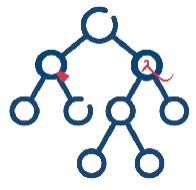
\includegraphics[height=1.0cm]{msca_logo.png}}%
    \end{center}

    \vspace{0.6cm}

    % Main title with Q logos on sides (with clickable links)
    \begin{center}
        \begin{minipage}{0.1\textwidth}
            \centering
            \href{https://quantlet.com}{
\includegraphics[height=1.1cm]{ql_logo.png}}
        \end{minipage}%
        \begin{minipage}{0.78\textwidth}
            \centering
            {\LARGE\bfseries\usebeamercolor[fg]{title}\inserttitle}

            \vspace{0.3cm}

            {\usebeamerfont{subtitle}\usebeamercolor[fg]{title}\insertsubtitle}
        \end{minipage}%
        \begin{minipage}{0.1\textwidth}
            \centering
            \href{https://quantinar.com}{
\includegraphics[height=1.1cm]{qr_logo.png}}
        \end{minipage}
    \end{center}

    \vspace{0.6cm}

    % Authors (left aligned)
    \hspace{0.5cm}{\usebeamerfont{author}\insertauthor}

    \vspace{0.3cm}

    % Institute/Affiliations (left aligned)
    \hspace{0.5cm}\begin{minipage}[t]{0.9\textwidth}
        \raggedright\small\insertinstitute
    \end{minipage}
}

%=============================================================================
% THEOREM ENVIRONMENTS
%=============================================================================
\theoremstyle{definition}
\setbeamertemplate{theorems}[numbered]
\ifdefined\atslang
\newtheorem{defn}{Definiție}
\newtheorem{thm}{Teoremă}
\newtheorem{prop}{Propoziție}
\newtheorem{rmk}{Observație}
\else
\newtheorem{defn}{Definition}
\newtheorem{thm}{Theorem}
\newtheorem{prop}{Proposition}
\newtheorem{rmk}{Remark}
\fi

%=============================================================================
% CENTRED MINIPAGE (no extra vertical space)
%=============================================================================
\newenvironment{cminipage}[1]{%
    \par\noindent\hfill\begin{minipage}{#1}\ignorespaces
}{%
    \end{minipage}\hfill\null\par
}

%=============================================================================
% CUSTOM COMMANDS
%=============================================================================
\newcommand{\E}{\mathbb{E}}
\newcommand{\Var}{\text{Var}}
\newcommand{\Cov}{\text{Cov}}
\newcommand{\Corr}{\text{Corr}}
\newcommand{\R}{\mathbb{R}}
\newcommand{\N}{\mathbb{N}}
\newcommand{\Z}{\mathbb{Z}}
\newcommand{\B}{\mathbf{B}}
\newcommand{\imark}{\textcolor{MainBlue}{\textbullet}}
\newcommand{\RMSE}{\text{RMSE}}
\newcommand{\MAE}{\text{MAE}}
\newcommand{\MAPE}{\text{MAPE}}

% Boldface vector/matrix commands (VAR, VECM, state space)
\newcommand{\bY}{\mathbf{Y}}
\newcommand{\bX}{\mathbf{X}}
\newcommand{\bA}{\mathbf{A}}
\newcommand{\bB}{\mathbf{B}}
\newcommand{\bepsilon}{\boldsymbol{\varepsilon}}
\newcommand{\bSigma}{\boldsymbol{\Sigma}}
\newcommand{\bPhi}{\boldsymbol{\Phi}}
\newcommand{\bGamma}{\boldsymbol{\Gamma}}
\newcommand{\bPi}{\boldsymbol{\Pi}}
\newcommand{\bc}{\mathbf{c}}
\newcommand{\balpha}{\boldsymbol{\alpha}}
\newcommand{\bbeta}{\boldsymbol{\beta}}
\newcommand{\bvarepsilon}{\boldsymbol{\varepsilon}}

% Seminar marks
\newcommand{\correct}{\textcolor{Forest}{\checkmark}}
\newcommand{\incorrect}{\textcolor{Crimson}{\texttimes}}
 se definește
%   \newcommand{\coursename}{Advanced Time Series Analysis and Forecasting}          (EN)
%   \newcommand{\coursename}{Analiza avansată a seriilor de timp și previziune}       (RO)  și  \def\atslang{ro}
% Fișierele .tex se află în EN/Courses, EN/Seminars, RO/Cursuri, RO/Seminarii (două niveluri sub rădăcină).
% Deck-urile sînt generate de latex/build_chapterN.py / build_seminarN.py (vezi latex/ats_build.py).

\documentclass[9pt, aspectratio=169, t]{beamer}
\providecommand{\coursename}{Advanced Time Series Analysis and Forecasting}

% Ensure content fits on slides
\setbeamersize{text margin left=8mm, text margin right=8mm}
% Smaller institute font (title page)
\setbeamerfont{institute}{size=\footnotesize}

%=============================================================================
% THEME AND STYLE CONFIGURATION
%=============================================================================
\usetheme{default}
% Using default theme for clean header/footer control

% Color Palette (matching Redispatch PDF)
\definecolor{MainBlue}{RGB}{26, 58, 110}
\definecolor{AccentBlue}{RGB}{26, 58, 110}
\definecolor{IDAred}{RGB}{205, 0, 0}
\definecolor{DarkGray}{RGB}{51, 51, 51}
\definecolor{MediumGray}{RGB}{128, 128, 128}
\definecolor{LightGray}{RGB}{248, 248, 248}
\definecolor{VeryLightGray}{RGB}{235, 235, 235}
\definecolor{KeynoteGray}{RGB}{218, 218, 218}
\definecolor{SectionGray}{RGB}{120, 120, 120}
\definecolor{FooterGray}{RGB}{100, 100, 100}
\definecolor{Crimson}{RGB}{220, 53, 69}
\definecolor{Forest}{RGB}{46, 125, 50}
\definecolor{Amber}{RGB}{181, 133, 63}
\definecolor{Orange}{RGB}{230, 126, 34}
\definecolor{Purple}{RGB}{142, 68, 173}

% Gradient background (exact Keynote 315° gradient: white to RGB 218,218,218)
\setbeamertemplate{background}{%
    \begin{tikzpicture}[remember picture, overlay]
        \shade[shading=axis, shading angle=315,
        top color=white, bottom color=KeynoteGray]
        (current page.south west) rectangle (current page.north east);
    \end{tikzpicture}%
}
% Fallback solid color for compatibility
\setbeamercolor{background canvas}{bg=}

\setbeamercolor{palette primary}{bg=MainBlue, fg=white}
\setbeamercolor{palette secondary}{bg=MainBlue!85, fg=white}
\setbeamercolor{palette tertiary}{bg=MainBlue!70, fg=white}
\setbeamercolor{structure}{fg=MainBlue}
\setbeamercolor{title}{fg=IDAred}
\setbeamercolor{frametitle}{fg=IDAred, bg=}
\setbeamercolor{block title}{bg=MainBlue, fg=white}
\setbeamercolor{block body}{bg=VeryLightGray, fg=DarkGray}
\setbeamercolor{block title alerted}{bg=Crimson, fg=white}
\setbeamercolor{block body alerted}{bg=Crimson!8, fg=DarkGray}
\setbeamercolor{block title example}{bg=Forest, fg=white}
\setbeamercolor{block body example}{bg=Forest!8, fg=DarkGray}
\setbeamercolor{item}{fg=MainBlue}

% Footer colors (override Madrid theme blue)
\setbeamercolor{author in head/foot}{fg=FooterGray, bg=}
\setbeamercolor{title in head/foot}{fg=FooterGray, bg=}
\setbeamercolor{date in head/foot}{fg=FooterGray, bg=}
\setbeamercolor{section in head/foot}{fg=FooterGray, bg=}
\setbeamercolor{subsection in head/foot}{fg=FooterGray, bg=}

% Bullet styles (apply everywhere including blocks)
\setbeamertemplate{itemize item}{\color{MainBlue}$\boxdot$}
\setbeamertemplate{itemize subitem}{\color{MainBlue}$\blacktriangleright$}
\setbeamertemplate{itemize subsubitem}{\color{MainBlue}\tiny$\bullet$}
\setbeamertemplate{itemize/enumerate body begin}{\normalsize}
\setbeamertemplate{itemize/enumerate subbody begin}{\normalsize}

% Item spacing - compact style
\setlength{\leftmargini}{10pt}       % Level 1: minimal indent
\setlength{\leftmarginii}{10pt}      % Level 2: minimal additional indent
% Compact list spacing (zero extra space before/after lists in blocks)
\makeatletter
\def\@listi{\leftmargin\leftmargini \topsep 0pt \parsep 0pt \itemsep 0pt}
\def\@listii{\leftmargin\leftmarginii \topsep 0pt \parsep 0pt \itemsep 0pt}
\makeatother

\setbeamertemplate{navigation symbols}{}

%=============================================================================
% CUSTOM HEADLINE
%=============================================================================
\setbeamertemplate{headline}{%
    \vskip10pt%
    \hbox to \paperwidth{%
        \hskip0.5cm%
        {\small\color{FooterGray}\renewcommand{\hyperlink}[2]{##2}\insertsectionhead}%
        \hfill%
        \textcolor{FooterGray}{\small\insertframenumber}%
        \hskip0.5cm%
    }%
    \vskip4pt%
    {\color{FooterGray}\hrule height 0.4pt}%
}

%=============================================================================
% CUSTOM FOOTER
%=============================================================================
\usepackage{fontawesome5}

\setbeamertemplate{footline}{%
    {\color{FooterGray}\hrule height 0.4pt}%
    \vskip4pt%
    \hbox to \paperwidth{%
        \hskip0.5cm%
        \textcolor{FooterGray}{\small\coursename}%
        \hfill%
        \raisebox{-0.1em}{%
            \begin{tikzpicture}[x=0.08em, y=0.08em, line width=0.4pt]
                \draw[FooterGray] (0,3) -- (1,4) -- (2,3.5) -- (3,5) -- (4,4) -- (5,6) -- (6,5.5) -- (7,4) -- (8,5) -- (9,7) -- (10,6) -- (11,5) -- (12,6.5) -- (13,8) -- (14,7) -- (15,6) -- (16,7.5) -- (17,9) -- (18,8) -- (19,7) -- (20,8.5) -- (21,10) -- (22,9) -- (23,8) -- (24,9.5);
            \end{tikzpicture}%
        }%
        \hskip0.5cm%
    }%
    \vskip6pt%
}

%=============================================================================
% PACKAGES
%=============================================================================
\usepackage[utf8]{inputenc}
\DeclareUnicodeCharacter{03B1}{\ensuremath{\alpha}}
\usepackage[T1]{fontenc}
\usepackage{amsmath, amssymb, amsthm}
\usepackage{mathtools}
\usepackage{bm}
\usepackage{tikz}
\usetikzlibrary{arrows.meta, positioning, shapes, calc, decorations.pathreplacing, shadings}
\usepackage{booktabs}
\usepackage{multirow}
\usepackage{array}
\usepackage{graphicx}
\usepackage{animate}
\usepackage{hyperref}
\usepackage{colortbl}
\usepackage{listings}
\lstset{language=Python, basicstyle=\ttfamily\scriptsize, keywordstyle=\color{MainBlue}\bfseries,
  commentstyle=\color{Forest}, stringstyle=\color{Crimson}, breaklines=true,
  frame=none, backgroundcolor=\color{VeryLightGray}, xleftmargin=2mm}
\hypersetup{colorlinks=true, linkcolor=MainBlue, urlcolor=MainBlue}
\graphicspath{{../../logos/}{../../charts/}{../../photos/}}
\usepackage{xcolor}
\hfuzz=2pt  % Suppress tiny overfull warnings (<2pt)
\vfuzz=2pt  % Suppress tiny vertical overfull warnings (<2pt)

%=============================================================================
% QUANTLET COMMANDS
%   \quantlet{<displayed name>}{<url>}       (generic)
%   \atsquantlet{Ch_05}{ATS_ch5_garch}       -> https://github.com/danpele/Advanced-Time-Series/tree/main/Quantlets/Ch_05/ATS_ch5_garch
%   \qlurl{<folder>} is defined per chapter by the generator (Quantlets/Ch_NN/<folder>)
%=============================================================================
\newcommand{\atsrepo}{https://github.com/danpele/Advanced-Time-Series}
\newcommand{\atsqlbase}{https://github.com/danpele/Advanced-Time-Series/tree/main/Quantlets}
\newcommand{\quantlet}[2]{%
    \hfill\href{#2}{%
        \raisebox{-0.15em}{
\includegraphics[height=0.7em]{ql_logo.png}}%
        \textcolor{MainBlue}{\tiny\ #1}%
    }%
}
\newcommand{\atsquantlet}[2]{\quantlet{\detokenize{#2}}{\atsqlbase/#1/#2}}

%=============================================================================
% NOTEBOOKS (Google Colab)
%   \colaburl{notebooks/EN/chapter5_seminar_notebook.ipynb} -> the Colab link of a file in the ATS repo
%   \nb: the chapter notebook (each seminar deck redefines it with \renewcommand)
%=============================================================================
\newcommand{\colaburl}[1]{https://colab.research.google.com/github/danpele/Advanced-Time-Series/blob/main/#1}
\newcommand{\nb}{https://colab.research.google.com/github/danpele/Advanced-Time-Series/tree/main/notebooks/EN}
\newcommand{\nbname}{notebooks/EN}

%=============================================================================
% SLIDE HELPERS (used by the generators; the same as in MFM)
%=============================================================================
% local font size for list bodies (the preamble forces \normalsize)
\newcommand{\itemsize}[1]{\setbeamertemplate{itemize/enumerate body begin}{#1}\setbeamertemplate{itemize/enumerate subbody begin}{#1}}
\newcommand{\intitle}[1]{{\hypersetup{urlcolor=white}#1}}   % white links inside coloured title bars
\newcommand{\imgcap}[1]{{\scriptsize #1}\\[0.5mm]}          % caption under a photo
\newcommand{\imgcredit}[2]{{\tiny\color{FooterGray}\href{#1}{#2}}}   % image credit: source URL, author/licence
\newcommand{\aiprompt}[1]{{\ttfamily\color{MainBlue}#1}}     % a prompt to an AI assistant

%=============================================================================
% SEMINARS: student version by default; the instructor wrapper *_solutions.tex sets \solutionstrue
%=============================================================================
\makeatletter\@ifundefined{ifsolutions}{\expandafter\newif\csname ifsolutions\endcsname}{}\makeatother
\newcommand{\solonly}[1]{\ifsolutions #1\fi}
\newcommand{\propsub}{\ifsolutions\else\framesubtitle{\ifdefined\atslang Rezolvarea se discută la seminar\else Solution discussed in class\fi}\fi}

%=============================================================================
% APPENDIX AND CHAPTER LINKS (latex/appendix_links.py writes the calls; it also re-declares these
% macros before \begin{document}, so the decks compile with or without this preamble block)
%=============================================================================
\providecommand{\atsapplink}[3]{\hypertarget{#2}{}\hyperlink{#1}{\beamergotobutton{#3}}}
\providecommand{\atsappback}[2]{\begin{tikzpicture}[remember picture,overlay]\node[anchor=south east] at ([xshift=-3mm,yshift=7mm]current page.south east){\hyperlink{#1}{\beamerreturnbutton{#2}}};\end{tikzpicture}}
\providecommand{\atschlink}[2]{\href{#1}{#2}}
\providecommand{\atschlinkt}[2]{\href{#1}{\usebeamercolor[fg]{frametitle}#2}}

%=============================================================================
% QUANTINAR COMMAND: link către un curs Quantinar (subiecte avansate)
%=============================================================================
\newcommand{\quantinar}[2]{%
    \href{#2}{%
        \raisebox{-0.15em}{
\includegraphics[height=0.8em]{qr_logo.png}}%
        \textcolor{MainBlue}{\scriptsize\ #1}%
    }%
}

%=============================================================================
% CUSTOM TITLE PAGE
%=============================================================================
\defbeamertemplate*{title page}{hybrid}[1][]
{
    \vspace{0.2cm}
    % Logos row - top header (with clickable links)
    \begin{center}
        \href{https://www.ase.ro}{
\includegraphics[height=1.0cm]{ase_logo.png}}\hspace{0.3cm}%
        \href{https://theida.net}{
\includegraphics[height=1.0cm]{ida_logo.png}}\hspace{0.3cm}%
        \href{https://blockchain-research-center.com}{
\includegraphics[height=1.0cm]{brc_logo.png}}\hspace{0.3cm}%
        \href{https://www.ai4efin.ase.ro}{
\includegraphics[height=1.0cm]{ai4efin_logo.png}}\hspace{0.3cm}%
        \href{https://ipe.ro/new}{
\includegraphics[height=1.0cm]{acad_logo.png}}\hspace{0.3cm}%
        \href{https://www.digital-finance-msca.com}{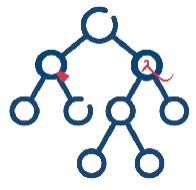
\includegraphics[height=1.0cm]{msca_logo.png}}%
    \end{center}

    \vspace{0.6cm}

    % Main title with Q logos on sides (with clickable links)
    \begin{center}
        \begin{minipage}{0.1\textwidth}
            \centering
            \href{https://quantlet.com}{
\includegraphics[height=1.1cm]{ql_logo.png}}
        \end{minipage}%
        \begin{minipage}{0.78\textwidth}
            \centering
            {\LARGE\bfseries\usebeamercolor[fg]{title}\inserttitle}

            \vspace{0.3cm}

            {\usebeamerfont{subtitle}\usebeamercolor[fg]{title}\insertsubtitle}
        \end{minipage}%
        \begin{minipage}{0.1\textwidth}
            \centering
            \href{https://quantinar.com}{
\includegraphics[height=1.1cm]{qr_logo.png}}
        \end{minipage}
    \end{center}

    \vspace{0.6cm}

    % Authors (left aligned)
    \hspace{0.5cm}{\usebeamerfont{author}\insertauthor}

    \vspace{0.3cm}

    % Institute/Affiliations (left aligned)
    \hspace{0.5cm}\begin{minipage}[t]{0.9\textwidth}
        \raggedright\small\insertinstitute
    \end{minipage}
}

%=============================================================================
% THEOREM ENVIRONMENTS
%=============================================================================
\theoremstyle{definition}
\setbeamertemplate{theorems}[numbered]
\ifdefined\atslang
\newtheorem{defn}{Definiție}
\newtheorem{thm}{Teoremă}
\newtheorem{prop}{Propoziție}
\newtheorem{rmk}{Observație}
\else
\newtheorem{defn}{Definition}
\newtheorem{thm}{Theorem}
\newtheorem{prop}{Proposition}
\newtheorem{rmk}{Remark}
\fi

%=============================================================================
% CENTRED MINIPAGE (no extra vertical space)
%=============================================================================
\newenvironment{cminipage}[1]{%
    \par\noindent\hfill\begin{minipage}{#1}\ignorespaces
}{%
    \end{minipage}\hfill\null\par
}

%=============================================================================
% CUSTOM COMMANDS
%=============================================================================
\newcommand{\E}{\mathbb{E}}
\newcommand{\Var}{\text{Var}}
\newcommand{\Cov}{\text{Cov}}
\newcommand{\Corr}{\text{Corr}}
\newcommand{\R}{\mathbb{R}}
\newcommand{\N}{\mathbb{N}}
\newcommand{\Z}{\mathbb{Z}}
\newcommand{\B}{\mathbf{B}}
\newcommand{\imark}{\textcolor{MainBlue}{\textbullet}}
\newcommand{\RMSE}{\text{RMSE}}
\newcommand{\MAE}{\text{MAE}}
\newcommand{\MAPE}{\text{MAPE}}

% Boldface vector/matrix commands (VAR, VECM, state space)
\newcommand{\bY}{\mathbf{Y}}
\newcommand{\bX}{\mathbf{X}}
\newcommand{\bA}{\mathbf{A}}
\newcommand{\bB}{\mathbf{B}}
\newcommand{\bepsilon}{\boldsymbol{\varepsilon}}
\newcommand{\bSigma}{\boldsymbol{\Sigma}}
\newcommand{\bPhi}{\boldsymbol{\Phi}}
\newcommand{\bGamma}{\boldsymbol{\Gamma}}
\newcommand{\bPi}{\boldsymbol{\Pi}}
\newcommand{\bc}{\mathbf{c}}
\newcommand{\balpha}{\boldsymbol{\alpha}}
\newcommand{\bbeta}{\boldsymbol{\beta}}
\newcommand{\bvarepsilon}{\boldsymbol{\varepsilon}}

% Seminar marks
\newcommand{\correct}{\textcolor{Forest}{\checkmark}}
\newcommand{\incorrect}{\textcolor{Crimson}{\texttimes}}
 se definește
%   \newcommand{\coursename}{Advanced Time Series Analysis and Forecasting}          (EN)
%   \newcommand{\coursename}{Analiza avansată a seriilor de timp și previziune}       (RO)  și  \def\atslang{ro}
% Fișierele .tex se află în EN/Courses, EN/Seminars, RO/Cursuri, RO/Seminarii (două niveluri sub rădăcină).
% Deck-urile sînt generate de latex/build_chapterN.py / build_seminarN.py (vezi latex/ats_build.py).

\documentclass[9pt, aspectratio=169, t]{beamer}
\providecommand{\coursename}{Advanced Time Series Analysis and Forecasting}

% Ensure content fits on slides
\setbeamersize{text margin left=8mm, text margin right=8mm}
% Smaller institute font (title page)
\setbeamerfont{institute}{size=\footnotesize}

%=============================================================================
% THEME AND STYLE CONFIGURATION
%=============================================================================
\usetheme{default}
% Using default theme for clean header/footer control

% Color Palette (matching Redispatch PDF)
\definecolor{MainBlue}{RGB}{26, 58, 110}
\definecolor{AccentBlue}{RGB}{26, 58, 110}
\definecolor{IDAred}{RGB}{205, 0, 0}
\definecolor{DarkGray}{RGB}{51, 51, 51}
\definecolor{MediumGray}{RGB}{128, 128, 128}
\definecolor{LightGray}{RGB}{248, 248, 248}
\definecolor{VeryLightGray}{RGB}{235, 235, 235}
\definecolor{KeynoteGray}{RGB}{218, 218, 218}
\definecolor{SectionGray}{RGB}{120, 120, 120}
\definecolor{FooterGray}{RGB}{100, 100, 100}
\definecolor{Crimson}{RGB}{220, 53, 69}
\definecolor{Forest}{RGB}{46, 125, 50}
\definecolor{Amber}{RGB}{181, 133, 63}
\definecolor{Orange}{RGB}{230, 126, 34}
\definecolor{Purple}{RGB}{142, 68, 173}

% Gradient background (exact Keynote 315° gradient: white to RGB 218,218,218)
\setbeamertemplate{background}{%
    \begin{tikzpicture}[remember picture, overlay]
        \shade[shading=axis, shading angle=315,
        top color=white, bottom color=KeynoteGray]
        (current page.south west) rectangle (current page.north east);
    \end{tikzpicture}%
}
% Fallback solid color for compatibility
\setbeamercolor{background canvas}{bg=}

\setbeamercolor{palette primary}{bg=MainBlue, fg=white}
\setbeamercolor{palette secondary}{bg=MainBlue!85, fg=white}
\setbeamercolor{palette tertiary}{bg=MainBlue!70, fg=white}
\setbeamercolor{structure}{fg=MainBlue}
\setbeamercolor{title}{fg=IDAred}
\setbeamercolor{frametitle}{fg=IDAred, bg=}
\setbeamercolor{block title}{bg=MainBlue, fg=white}
\setbeamercolor{block body}{bg=VeryLightGray, fg=DarkGray}
\setbeamercolor{block title alerted}{bg=Crimson, fg=white}
\setbeamercolor{block body alerted}{bg=Crimson!8, fg=DarkGray}
\setbeamercolor{block title example}{bg=Forest, fg=white}
\setbeamercolor{block body example}{bg=Forest!8, fg=DarkGray}
\setbeamercolor{item}{fg=MainBlue}

% Footer colors (override Madrid theme blue)
\setbeamercolor{author in head/foot}{fg=FooterGray, bg=}
\setbeamercolor{title in head/foot}{fg=FooterGray, bg=}
\setbeamercolor{date in head/foot}{fg=FooterGray, bg=}
\setbeamercolor{section in head/foot}{fg=FooterGray, bg=}
\setbeamercolor{subsection in head/foot}{fg=FooterGray, bg=}

% Bullet styles (apply everywhere including blocks)
\setbeamertemplate{itemize item}{\color{MainBlue}$\boxdot$}
\setbeamertemplate{itemize subitem}{\color{MainBlue}$\blacktriangleright$}
\setbeamertemplate{itemize subsubitem}{\color{MainBlue}\tiny$\bullet$}
\setbeamertemplate{itemize/enumerate body begin}{\normalsize}
\setbeamertemplate{itemize/enumerate subbody begin}{\normalsize}

% Item spacing - compact style
\setlength{\leftmargini}{10pt}       % Level 1: minimal indent
\setlength{\leftmarginii}{10pt}      % Level 2: minimal additional indent
% Compact list spacing (zero extra space before/after lists in blocks)
\makeatletter
\def\@listi{\leftmargin\leftmargini \topsep 0pt \parsep 0pt \itemsep 0pt}
\def\@listii{\leftmargin\leftmarginii \topsep 0pt \parsep 0pt \itemsep 0pt}
\makeatother

\setbeamertemplate{navigation symbols}{}

%=============================================================================
% CUSTOM HEADLINE
%=============================================================================
\setbeamertemplate{headline}{%
    \vskip10pt%
    \hbox to \paperwidth{%
        \hskip0.5cm%
        {\small\color{FooterGray}\renewcommand{\hyperlink}[2]{##2}\insertsectionhead}%
        \hfill%
        \textcolor{FooterGray}{\small\insertframenumber}%
        \hskip0.5cm%
    }%
    \vskip4pt%
    {\color{FooterGray}\hrule height 0.4pt}%
}

%=============================================================================
% CUSTOM FOOTER
%=============================================================================
\usepackage{fontawesome5}

\setbeamertemplate{footline}{%
    {\color{FooterGray}\hrule height 0.4pt}%
    \vskip4pt%
    \hbox to \paperwidth{%
        \hskip0.5cm%
        \textcolor{FooterGray}{\small\coursename}%
        \hfill%
        \raisebox{-0.1em}{%
            \begin{tikzpicture}[x=0.08em, y=0.08em, line width=0.4pt]
                \draw[FooterGray] (0,3) -- (1,4) -- (2,3.5) -- (3,5) -- (4,4) -- (5,6) -- (6,5.5) -- (7,4) -- (8,5) -- (9,7) -- (10,6) -- (11,5) -- (12,6.5) -- (13,8) -- (14,7) -- (15,6) -- (16,7.5) -- (17,9) -- (18,8) -- (19,7) -- (20,8.5) -- (21,10) -- (22,9) -- (23,8) -- (24,9.5);
            \end{tikzpicture}%
        }%
        \hskip0.5cm%
    }%
    \vskip6pt%
}

%=============================================================================
% PACKAGES
%=============================================================================
\usepackage[utf8]{inputenc}
\DeclareUnicodeCharacter{03B1}{\ensuremath{\alpha}}
\usepackage[T1]{fontenc}
\usepackage{amsmath, amssymb, amsthm}
\usepackage{mathtools}
\usepackage{bm}
\usepackage{tikz}
\usetikzlibrary{arrows.meta, positioning, shapes, calc, decorations.pathreplacing, shadings}
\usepackage{booktabs}
\usepackage{multirow}
\usepackage{array}
\usepackage{graphicx}
\usepackage{animate}
\usepackage{hyperref}
\usepackage{colortbl}
\usepackage{listings}
\lstset{language=Python, basicstyle=\ttfamily\scriptsize, keywordstyle=\color{MainBlue}\bfseries,
  commentstyle=\color{Forest}, stringstyle=\color{Crimson}, breaklines=true,
  frame=none, backgroundcolor=\color{VeryLightGray}, xleftmargin=2mm}
\hypersetup{colorlinks=true, linkcolor=MainBlue, urlcolor=MainBlue}
\graphicspath{{../../logos/}{../../charts/}{../../photos/}}
\usepackage{xcolor}
\hfuzz=2pt  % Suppress tiny overfull warnings (<2pt)
\vfuzz=2pt  % Suppress tiny vertical overfull warnings (<2pt)

%=============================================================================
% QUANTLET COMMANDS
%   \quantlet{<displayed name>}{<url>}       (generic)
%   \atsquantlet{Ch_05}{ATS_ch5_garch}       -> https://github.com/danpele/Advanced-Time-Series/tree/main/Quantlets/Ch_05/ATS_ch5_garch
%   \qlurl{<folder>} is defined per chapter by the generator (Quantlets/Ch_NN/<folder>)
%=============================================================================
\newcommand{\atsrepo}{https://github.com/danpele/Advanced-Time-Series}
\newcommand{\atsqlbase}{https://github.com/danpele/Advanced-Time-Series/tree/main/Quantlets}
\newcommand{\quantlet}[2]{%
    \hfill\href{#2}{%
        \raisebox{-0.15em}{
\includegraphics[height=0.7em]{ql_logo.png}}%
        \textcolor{MainBlue}{\tiny\ #1}%
    }%
}
\newcommand{\atsquantlet}[2]{\quantlet{\detokenize{#2}}{\atsqlbase/#1/#2}}

%=============================================================================
% NOTEBOOKS (Google Colab)
%   \colaburl{notebooks/EN/chapter5_seminar_notebook.ipynb} -> the Colab link of a file in the ATS repo
%   \nb: the chapter notebook (each seminar deck redefines it with \renewcommand)
%=============================================================================
\newcommand{\colaburl}[1]{https://colab.research.google.com/github/danpele/Advanced-Time-Series/blob/main/#1}
\newcommand{\nb}{https://colab.research.google.com/github/danpele/Advanced-Time-Series/tree/main/notebooks/EN}
\newcommand{\nbname}{notebooks/EN}

%=============================================================================
% SLIDE HELPERS (used by the generators; the same as in MFM)
%=============================================================================
% local font size for list bodies (the preamble forces \normalsize)
\newcommand{\itemsize}[1]{\setbeamertemplate{itemize/enumerate body begin}{#1}\setbeamertemplate{itemize/enumerate subbody begin}{#1}}
\newcommand{\intitle}[1]{{\hypersetup{urlcolor=white}#1}}   % white links inside coloured title bars
\newcommand{\imgcap}[1]{{\scriptsize #1}\\[0.5mm]}          % caption under a photo
\newcommand{\imgcredit}[2]{{\tiny\color{FooterGray}\href{#1}{#2}}}   % image credit: source URL, author/licence
\newcommand{\aiprompt}[1]{{\ttfamily\color{MainBlue}#1}}     % a prompt to an AI assistant

%=============================================================================
% SEMINARS: student version by default; the instructor wrapper *_solutions.tex sets \solutionstrue
%=============================================================================
\makeatletter\@ifundefined{ifsolutions}{\expandafter\newif\csname ifsolutions\endcsname}{}\makeatother
\newcommand{\solonly}[1]{\ifsolutions #1\fi}
\newcommand{\propsub}{\ifsolutions\else\framesubtitle{\ifdefined\atslang Rezolvarea se discută la seminar\else Solution discussed in class\fi}\fi}

%=============================================================================
% APPENDIX AND CHAPTER LINKS (latex/appendix_links.py writes the calls; it also re-declares these
% macros before \begin{document}, so the decks compile with or without this preamble block)
%=============================================================================
\providecommand{\atsapplink}[3]{\hypertarget{#2}{}\hyperlink{#1}{\beamergotobutton{#3}}}
\providecommand{\atsappback}[2]{\begin{tikzpicture}[remember picture,overlay]\node[anchor=south east] at ([xshift=-3mm,yshift=7mm]current page.south east){\hyperlink{#1}{\beamerreturnbutton{#2}}};\end{tikzpicture}}
\providecommand{\atschlink}[2]{\href{#1}{#2}}
\providecommand{\atschlinkt}[2]{\href{#1}{\usebeamercolor[fg]{frametitle}#2}}

%=============================================================================
% QUANTINAR COMMAND: link către un curs Quantinar (subiecte avansate)
%=============================================================================
\newcommand{\quantinar}[2]{%
    \href{#2}{%
        \raisebox{-0.15em}{
\includegraphics[height=0.8em]{qr_logo.png}}%
        \textcolor{MainBlue}{\scriptsize\ #1}%
    }%
}

%=============================================================================
% CUSTOM TITLE PAGE
%=============================================================================
\defbeamertemplate*{title page}{hybrid}[1][]
{
    \vspace{0.2cm}
    % Logos row - top header (with clickable links)
    \begin{center}
        \href{https://www.ase.ro}{
\includegraphics[height=1.0cm]{ase_logo.png}}\hspace{0.3cm}%
        \href{https://theida.net}{
\includegraphics[height=1.0cm]{ida_logo.png}}\hspace{0.3cm}%
        \href{https://blockchain-research-center.com}{
\includegraphics[height=1.0cm]{brc_logo.png}}\hspace{0.3cm}%
        \href{https://www.ai4efin.ase.ro}{
\includegraphics[height=1.0cm]{ai4efin_logo.png}}\hspace{0.3cm}%
        \href{https://ipe.ro/new}{
\includegraphics[height=1.0cm]{acad_logo.png}}\hspace{0.3cm}%
        \href{https://www.digital-finance-msca.com}{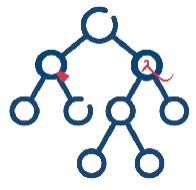
\includegraphics[height=1.0cm]{msca_logo.png}}%
    \end{center}

    \vspace{0.6cm}

    % Main title with Q logos on sides (with clickable links)
    \begin{center}
        \begin{minipage}{0.1\textwidth}
            \centering
            \href{https://quantlet.com}{
\includegraphics[height=1.1cm]{ql_logo.png}}
        \end{minipage}%
        \begin{minipage}{0.78\textwidth}
            \centering
            {\LARGE\bfseries\usebeamercolor[fg]{title}\inserttitle}

            \vspace{0.3cm}

            {\usebeamerfont{subtitle}\usebeamercolor[fg]{title}\insertsubtitle}
        \end{minipage}%
        \begin{minipage}{0.1\textwidth}
            \centering
            \href{https://quantinar.com}{
\includegraphics[height=1.1cm]{qr_logo.png}}
        \end{minipage}
    \end{center}

    \vspace{0.6cm}

    % Authors (left aligned)
    \hspace{0.5cm}{\usebeamerfont{author}\insertauthor}

    \vspace{0.3cm}

    % Institute/Affiliations (left aligned)
    \hspace{0.5cm}\begin{minipage}[t]{0.9\textwidth}
        \raggedright\small\insertinstitute
    \end{minipage}
}

%=============================================================================
% THEOREM ENVIRONMENTS
%=============================================================================
\theoremstyle{definition}
\setbeamertemplate{theorems}[numbered]
\ifdefined\atslang
\newtheorem{defn}{Definiție}
\newtheorem{thm}{Teoremă}
\newtheorem{prop}{Propoziție}
\newtheorem{rmk}{Observație}
\else
\newtheorem{defn}{Definition}
\newtheorem{thm}{Theorem}
\newtheorem{prop}{Proposition}
\newtheorem{rmk}{Remark}
\fi

%=============================================================================
% CENTRED MINIPAGE (no extra vertical space)
%=============================================================================
\newenvironment{cminipage}[1]{%
    \par\noindent\hfill\begin{minipage}{#1}\ignorespaces
}{%
    \end{minipage}\hfill\null\par
}

%=============================================================================
% CUSTOM COMMANDS
%=============================================================================
\newcommand{\E}{\mathbb{E}}
\newcommand{\Var}{\text{Var}}
\newcommand{\Cov}{\text{Cov}}
\newcommand{\Corr}{\text{Corr}}
\newcommand{\R}{\mathbb{R}}
\newcommand{\N}{\mathbb{N}}
\newcommand{\Z}{\mathbb{Z}}
\newcommand{\B}{\mathbf{B}}
\newcommand{\imark}{\textcolor{MainBlue}{\textbullet}}
\newcommand{\RMSE}{\text{RMSE}}
\newcommand{\MAE}{\text{MAE}}
\newcommand{\MAPE}{\text{MAPE}}

% Boldface vector/matrix commands (VAR, VECM, state space)
\newcommand{\bY}{\mathbf{Y}}
\newcommand{\bX}{\mathbf{X}}
\newcommand{\bA}{\mathbf{A}}
\newcommand{\bB}{\mathbf{B}}
\newcommand{\bepsilon}{\boldsymbol{\varepsilon}}
\newcommand{\bSigma}{\boldsymbol{\Sigma}}
\newcommand{\bPhi}{\boldsymbol{\Phi}}
\newcommand{\bGamma}{\boldsymbol{\Gamma}}
\newcommand{\bPi}{\boldsymbol{\Pi}}
\newcommand{\bc}{\mathbf{c}}
\newcommand{\balpha}{\boldsymbol{\alpha}}
\newcommand{\bbeta}{\boldsymbol{\beta}}
\newcommand{\bvarepsilon}{\boldsymbol{\varepsilon}}

% Seminar marks
\newcommand{\correct}{\textcolor{Forest}{\checkmark}}
\newcommand{\incorrect}{\textcolor{Crimson}{\texttimes}}


\newcommand{\qlurl}[1]{https://github.com/danpele/Advanced-Time-Series/tree/main/Quantlets/Ch_15/#1}

% Clickable citations (DOIs verified via Crossref)
\newcommand{\refNW}{\href{https://doi.org/10.2307/1913610}{Newey and West (1987)}}
\newcommand{\refEH}{\href{https://doi.org/10.1111/j.1540-6261.1991.tb02674.x}{Estrella and Hardouvelis (1991)}}
\newcommand{\refWhite}{\href{https://doi.org/10.1111/1468-0262.00152}{White (2000)}}
\newcommand{\refMR}{\href{https://doi.org/10.1016/0022-1996(83)90017-X}{Meese and Rogoff (1983)}}
\newcommand{\refGKMT}{\href{https://doi.org/10.1016/j.ijforecast.2012.06.004}{Genre et al.\ (2013)}}
\newcommand{\refAO}{\href{https://doi.org/10.21034/qr.2511}{Atkeson and Ohanian (2001)}}
\newcommand{\refDM}{\href{https://doi.org/10.1080/07350015.1995.10524599}{Diebold and Mariano (1995)}}
\newcommand{\refHLN}{\href{https://doi.org/10.1016/S0169-2070(96)00719-4}{Harvey, Leybourne and Newbold (1997)}}
\newcommand{\refCW}{\href{https://doi.org/10.1016/j.jeconom.2006.05.023}{Clark and West (2007)}}
\newcommand{\refMPQ}{\href{https://doi.org/10.1257/aer.90.5.1464}{McConnell and Perez-Quiros (2000)}}
\newcommand{\refBP}{\href{https://doi.org/10.1002/jae.659}{Bai and Perron (2003)}}
\newcommand{\refHanB}{\href{https://doi.org/10.2202/1558-3708.1024}{Hansen (1997)}}
\newcommand{\refTPS}{\href{https://doi.org/10.1111/1468-2354.00144}{Taylor, Peel and Sarno (2001)}}
\newcommand{\refCEE}{\href{https://doi.org/10.1016/S1574-0048(99)01005-8}{Christiano, Eichenbaum and Evans (1999)}}
\newcommand{\refGK}{\href{https://doi.org/10.1257/mac.20130329}{Gertler and Karadi (2015)}}
\newcommand{\refKil}{\href{https://doi.org/10.1257/aer.99.3.1053}{Kilian (2009)}}
\newcommand{\refKPSW}{\href{https://www.jstor.org/stable/2006644}{King, Plosser, Stock and Watson (1991)}}
\newcommand{\refPSS}{\href{https://doi.org/10.1080/01621459.1999.10474156}{Pesaran, Shin and Smith (1999)}}
\newcommand{\refBGR}{\href{https://doi.org/10.1002/jae.1137}{Bańbura, Giannone and Reichlin (2010)}}
\newcommand{\refSW}{\href{https://doi.org/10.1198/073500102317351921}{Stock and Watson (2002)}}
\newcommand{\refMNZ}{\href{https://doi.org/10.1162/003465303765299765}{Morley, Nelson and Zivot (2003)}}
\newcommand{\refHam}{\href{https://doi.org/10.2307/1912559}{Hamilton (1989)}}
\newcommand{\refEGS}{\href{https://doi.org/10.1162/REST_a_00300}{Engle, Ghysels and Sohn (2013)}}
\newcommand{\refBPQ}{\href{https://doi.org/10.1016/j.jeconom.2015.10.007}{Bollerslev, Patton and Quaedvlieg (2016)}}
\newcommand{\refELW}{\href{https://doi.org/10.1080/07350015.2017.1345683}{Engle, Ledoit and Wolf (2019)}}
\newcommand{\refPZC}{\href{https://doi.org/10.1016/j.jeconom.2018.10.008}{Patton, Ziegel and Chen (2019)}}
\newcommand{\refEM}{\href{https://doi.org/10.1198/073500104000000370}{Engle and Manganelli (2004)}}
\newcommand{\refGJR}{\href{https://doi.org/10.1080/14697688.2017.1393551}{Gatheral, Jaisson and Rosenbaum (2018)}}
\newcommand{\refQu}{\href{https://doi.org/10.1198/jbes.2010.09153}{Qu (2011)}}
\newcommand{\refCN}{\href{https://doi.org/10.1016/0165-1889(93)00781-X}{Cogley and Nason (1995)}}
\newcommand{\refHamB}{\href{https://doi.org/10.1162/rest_a_00706}{Hamilton (2018)}}
\newcommand{\refBHK}{\href{https://doi.org/10.1016/j.csda.2017.11.003}{Bergmeir, Hyndman and Koo (2018)}}
\newcommand{\refZeng}{\href{https://doi.org/10.1609/aaai.v37i9.26317}{Zeng et al.\ (2023)}}
\newcommand{\refNie}{\href{https://arxiv.org/abs/2211.14730}{Nie et al.\ (2023)}}
\newcommand{\refGC}{\href{https://arxiv.org/abs/2106.00170}{Gibbs and Candès (2021)}}
\newcommand{\refRPC}{\href{https://arxiv.org/abs/1905.03222}{Romano, Patterson and Candès (2019)}}
\newcommand{\refADH}{\href{https://doi.org/10.1111/ajps.12116}{Abadie, Diamond and Hainmueller (2015)}}
\newcommand{\refBMSS}{\href{https://doi.org/10.1093/ej/uez020}{Born et al.\ (2019)}}
\newcommand{\refPWY}{\href{https://doi.org/10.1111/j.1468-2354.2010.00625.x}{Phillips, Wu and Yu (2011)}}
\newcommand{\refPSY}{\href{https://doi.org/10.1111/iere.12132}{Phillips, Shi and Yu (2015)}}
\newcommand{\refPY}{\href{https://doi.org/10.3982/QE82}{Phillips and Yu (2011)}}
\newcommand{\refHLST}{\href{https://doi.org/10.1016/j.jempfin.2015.09.002}{Harvey et al.\ (2016)}}
\newcommand{\refHansen}{\href{https://doi.org/10.1198/073500105000000063}{Hansen (2005)}}
\newcommand{\refHLNa}{\href{https://doi.org/10.3982/ECTA5771}{Hansen, Lunde and Nason (2011)}}
\newcommand{\refRW}{\href{https://doi.org/10.1111/j.1468-0262.2005.00615.x}{Romano and Wolf (2005)}}
\newcommand{\refKV}{\href{https://doi.org/10.1017/S0266466605050565}{Kiefer and Vogelsang (2005)}}
\newcommand{\refLLSW}{\href{https://doi.org/10.1080/07350015.2018.1506926}{Lazarus et al.\ (2018)}}
\newcommand{\refIK}{\href{https://doi.org/10.1081/ETC-200040785}{Inoue and Kilian (2005)}}
\newcommand{\refDiebold}{\href{https://doi.org/10.1080/07350015.2014.983236}{Diebold (2015)}}
\newcommand{\refStam}{\href{https://doi.org/10.1016/S0304-405X(99)00041-0}{Stambaugh (1999)}}
\newcommand{\refWG}{\href{https://doi.org/10.1093/rfs/hhm014}{Welch and Goyal (2008)}}
\newcommand{\refSNS}{\href{https://doi.org/10.1177/0956797611417632}{Simmons, Nelson and Simonsohn (2011)}}
\newcommand{\refGL}{\href{https://doi.org/10.1511/2014.111.460}{Gelman and Loken (2014)}}
\newcommand{\refHLZ}{\href{https://doi.org/10.1093/rfs/hhv059}{Harvey, Liu and Zhu (2016)}}
\newcommand{\refIoa}{\href{https://doi.org/10.1371/journal.pmed.0020124}{Ioannidis (2005)}}
\newcommand{\refBLSZ}{\href{https://doi.org/10.1257/app.20150044}{Brodeur et al.\ (2016)}}
\newcommand{\refNos}{\href{https://doi.org/10.1073/pnas.1708274114}{Nosek et al.\ (2018)}}
\newcommand{\refKau}{\href{https://doi.org/10.1145/2382577.2382579}{Kaufman et al.\ (2012)}}
\newcommand{\refCle}{\href{https://doi.org/10.1111/joes.12139}{Clemens (2017)}}
\newcommand{\refCM}{\href{https://doi.org/10.1257/jel.20171350}{Christensen and Miguel (2018)}}
\newcommand{\refVil}{\href{https://doi.org/10.1162/99608f92.4f6b9e67}{Vilhuber (2020)}}
\newcommand{\refCL}{\href{https://doi.org/10.1561/104.00000053}{Chang and Li (2022)}}
\newcommand{\refHAP}{\href{https://doi.org/10.1093/cje/bet075}{Herndon, Ash and Pollin (2014)}}
\newcommand{\refHXZ}{\href{https://doi.org/10.1093/rfs/hhy131}{Hou, Xue and Zhang (2020)}}
\newcommand{\refMen}{\href{https://doi.org/10.1111/jofi.13337}{Menkveld et al.\ (2024)}}
\newcommand{\refSil}{\href{https://doi.org/10.1177/2515245917747646}{Silberzahn et al.\ (2018)}}
\newcommand{\refSSN}{\href{https://doi.org/10.1038/s41562-020-0912-z}{Simonsohn, Simmons and Nelson (2020)}}
\newcommand{\refSte}{\href{https://doi.org/10.1177/1745691616658637}{Steegen et al.\ (2016)}}
\newcommand{\refPeng}{\href{https://doi.org/10.1126/science.1213847}{Peng (2011)}}
\newcommand{\refPet}{\href{https://doi.org/10.1016/j.ijforecast.2021.11.001}{Petropoulos et al.\ (2022)}}
\newcommand{\refMC}{\href{https://doi.org/10.1038/s41586-024-07146-0}{Messeri and Crockett (2024)}}
\newcommand{\refWW}{\href{https://doi.org/10.1038/s41598-023-41032-5}{Walters and Wilder (2023)}}
\newcommand{\refKor}{\href{https://doi.org/10.1257/jel.20231736}{Korinek (2023)}}
\newcommand{\refWang}{\href{https://doi.org/10.1038/s41586-023-06221-2}{Wang et al.\ (2023)}}
\newcommand{\refLu}{\href{https://arxiv.org/abs/2408.06292}{Lu et al.\ (2024)}}

\title[Advanced Time Series Analysis and Forecasting]{Advanced Time Series Analysis and Forecasting}
\subtitle{Chapter 15: Review and project defence}
\author[D.T. Pele]{Daniel Traian PELE}
\institute{Bucharest University of Economic Studies\\
IDA Institute Digital Assets\\
Blockchain Research Center\\
AI4EFin Artificial Intelligence for Energy Finance\\
Romanian Academy, Institute for Economic Forecasting\\
MSCA Digital Finance}
\date{}

%=============================================================================
\providecommand{\atsapplink}[3]{\hypertarget{#2}{}\hyperlink{#1}{\beamergotobutton{#3}}}  % APPLINKS-MACROS
\providecommand{\atsappback}[2]{\begin{tikzpicture}[remember picture,overlay]\node[anchor=south east] at ([xshift=-3mm,yshift=7mm]current page.south east){\hyperlink{#1}{\beamerreturnbutton{#2}}};\end{tikzpicture}}  % APPLINKS-MACROS
\providecommand{\atschlink}[2]{\href{#1}{#2}}  % APPLINKS-MACROS
\providecommand{\atschlinkt}[2]{\href{#1}{\usebeamercolor[fg]{frametitle}#2}}  % APPLINKS-MACROS
\begin{document}
%=============================================================================

{
\setbeamertemplate{headline}{}
\setbeamertemplate{footline}{}
\begin{frame}[noframenumbering]
    \titlepage
\end{frame}
}
% BEGIN-ACRONYMS (generat de latex/acronyms.py; nu editati manual)
\begin{frame}{Acronyms used in this material (1/4)}
\setbeamertemplate{itemize/enumerate body begin}{\tiny}
\begin{columns}[T]
\begin{column}{0.49\textwidth}
\begin{itemize}\setlength{\itemsep}{0pt}
    \item \textbf{ACI}: Adaptive Conformal Inference
    \item \textbf{AI}: Artificial Intelligence
    \item \textbf{ALFRED}: ArchivaL Federal Reserve Economic Data
    \item \textbf{AR}: AutoRegressive (model); in event studies: Abnormal Return
    \item \textbf{ARDL}: AutoRegressive Distributed Lag (model)
    \item \textbf{ARX}: AutoRegressive model with eXogenous variables
    \item \textbf{BET}: Bucharest Exchange Trading (index)
    \item \textbf{BH}: Benjamini–Hochberg (procedure)
    \item \textbf{BNR}: Banca Națională a României (the National Bank of Romania)
    \item \textbf{BSADF}: Backward Supremum Augmented Dickey–Fuller (statistic)
    \item \textbf{BVAR}: Bayesian Vector AutoRegression
    \item \textbf{CCE}: Common Correlated Effects (estimator)
    \item \textbf{CCM}: Convergent Cross Mapping
\end{itemize}
\end{column}
\begin{column}{0.49\textwidth}
\begin{itemize}\setlength{\itemsep}{0pt}
    \item \textbf{CEE}: Central and Eastern Europe
    \item \textbf{CPI}: Consumer Price Index
    \item \textbf{CQR}: Conformalized Quantile Regression
    \item \textbf{CRPS}: Continuous Ranked Probability Score
    \item \textbf{CSW}: Chu, Stinchcombe and White (monitoring boundary)
    \item \textbf{CV}: Cross-Validation
    \item \textbf{DCC}: Dynamic Conditional Correlation
    \item \textbf{DCC-NL}: DCC with Nonlinear shrinkage of the target (Engle–Ledoit–Wolf 2019)
    \item \textbf{DFM}: Dynamic Factor Model
    \item \textbf{DM}: Diebold–Mariano (test)
    \item \textbf{DQ}: Dynamic Quantile (test of Engle and Manganelli)
    \item \textbf{ECB}: European Central Bank
    \item \textbf{EM}: Expectation–Maximisation (algorithm)
\end{itemize}
\end{column}
\end{columns}
\end{frame}
\begin{frame}{Acronyms used in this material (2/4)}
\setbeamertemplate{itemize/enumerate body begin}{\tiny}
\begin{columns}[T]
\begin{column}{0.49\textwidth}
\begin{itemize}\setlength{\itemsep}{0pt}
    \item \textbf{EODHD}: EOD Historical Data (market-data provider)
    \item \textbf{ES}: Expected Shortfall
    \item \textbf{EU}: European Union
    \item \textbf{EU-27}: the 27 member states of the European Union
    \item \textbf{EWC}: Equal-Weighted Cosine (estimator)
    \item \textbf{FRED}: Federal Reserve Economic Data
    \item \textbf{FZ0}: Zero-homogeneous Fissler–Ziegel loss (Patton, Ziegel and Chen)
    \item \textbf{GARCH}: Generalised AutoRegressive Conditional Heteroskedasticity
    \item \textbf{GAS-1F}: One-factor GAS model for VaR and ES
    \item \textbf{GDP}: Gross Domestic Product
    \item \textbf{GMV}: Global Minimum-Variance (portfolio)
    \item \textbf{GSADF}: Generalised Supremum Augmented Dickey–Fuller (test)
    \item \textbf{HAC}: Heteroskedasticity and Autocorrelation Consistent (standard errors)
\end{itemize}
\end{column}
\begin{column}{0.49\textwidth}
\begin{itemize}\setlength{\itemsep}{0pt}
    \item \textbf{HAR}: Heterogeneous AutoRegressive (model)
    \item \textbf{HARQ}: HAR with realised Quarticity
    \item \textbf{HLN}: Harvey–Leybourne–Newbold (small-sample correction of the DM test)
    \item \textbf{HP}: Hodrick–Prescott (filter)
    \item \textbf{IG}: inverse gamma (distribution)
    \item \textbf{INS}: Institutul Național de Statistică (the National Institute of Statistics (Romania))
    \item \textbf{ITS}: Interrupted Time Series
    \item \textbf{LLM}: Large Language Model
    \item \textbf{LM}: Lagrange Multiplier
    \item \textbf{LP}: Local Projection
    \item \textbf{LP-IV}: Local Projection with Instrumental Variables
    \item \textbf{LR}: Likelihood Ratio (test)
    \item \textbf{MAE}: Mean Absolute Error
\end{itemize}
\end{column}
\end{columns}
\end{frame}
\begin{frame}{Acronyms used in this material (3/4)}
\setbeamertemplate{itemize/enumerate body begin}{\tiny}
\begin{columns}[T]
\begin{column}{0.49\textwidth}
\begin{itemize}\setlength{\itemsep}{0pt}
    \item \textbf{MCS}: Model Confidence Set
    \item \textbf{MGARCH}: Multivariate GARCH
    \item \textbf{MIDAS}: MIxed DAta Sampling (regression)
    \item \textbf{ML}: Machine Learning
    \item \textbf{MNZ}: Morley–Nelson–Zivot (2003)
    \item \textbf{MSE}: Mean Squared Error
    \item \textbf{MSFE}: Mean Squared Forecast Error
    \item \textbf{OECD}: Organisation for Economic Co-operation and Development
    \item \textbf{OLS}: Ordinary Least Squares
    \item \textbf{PCMCI}: PC algorithm + Momentary Conditional Independence
    \item \textbf{PID}: Proportional--Integral--Derivative (controller)
    \item \textbf{PIT}: Probability Integral Transform
    \item \textbf{PMG}: Pooled Mean Group (estimator)
\end{itemize}
\end{column}
\begin{column}{0.49\textwidth}
\begin{itemize}\setlength{\itemsep}{0pt}
    \item \textbf{QLIKE}: Quasi-LIKElihood loss
    \item \textbf{QML}: Quasi-Maximum Likelihood
    \item \textbf{QPS}: Quadratic Probability Score
    \item \textbf{RMSE}: Root Mean Squared Error
    \item \textbf{SAV}: Symmetric Absolute Value (CAViaR specification)
    \item \textbf{SC}: Synthetic Control
    \item \textbf{SPA}: Superior Predictive Ability (test)
    \item \textbf{SPF}: Survey of Professional Forecasters
    \item \textbf{STAR}: Smooth Transition AutoRegression
    \item \textbf{SVAR}: Structural Vector AutoRegression
    \item \textbf{TAR}: Threshold AutoRegression
    \item \textbf{TE}: Transfer Entropy
    \item \textbf{TPS}: Taylor, Peel and Sarno (2001)
\end{itemize}
\end{column}
\end{columns}
\end{frame}
\begin{frame}{Acronyms used in this material (4/4)}
\setbeamertemplate{itemize/enumerate body begin}{\tiny}
\begin{columns}[T]
\begin{column}{0.49\textwidth}
\begin{itemize}\setlength{\itemsep}{0pt}
    \item \textbf{UC-SV}: Unobserved Components model with Stochastic Volatility (Stock–Watson 2007)
    \item \textbf{UC0}: UC model with uncorrelated trend and cycle shocks (Clark 1987)
    \item \textbf{UK}: United Kingdom
    \item \textbf{US}: United States
    \item \textbf{VAR}: Vector AutoRegression
    \item \textbf{VECM}: Vector Error Correction Model
\end{itemize}
\end{column}
\begin{column}{0.49\textwidth}
\end{column}
\end{columns}
\end{frame}
% END-ACRONYMS

\begin{frame}{Today's question and route}
\itemsize{\small}
\begin{columns}[T]
\begin{column}{0.58\textwidth}
\begin{itemize}
    \item \textbf{Question}: what does the whole course give you for a research project, and how is the project defended?
    \begin{itemize}
        \item one chapter that ties \atschlink{https://danpele.github.io/Advanced-Time-Series/EN/Courses/chapter0_refresher_inference.pdf}{Chapters 0}--\atschlink{https://danpele.github.io/Advanced-Time-Series/EN/Courses/chapter14_causal_inference_time_series.pdf}{14} and the self-study \atschlink{https://danpele.github.io/Advanced-Time-Series/EN/Courses/chapter16_explosive_roots_bubbles.pdf}{Chapter 16} to the team project
    \end{itemize}
    \item \textbf{Route}
    \begin{itemize}
        \item Part I: the course map, one recap per chapter, the toolbox of methods
        \item Part II: the research workflow, how to replicate a landmark paper, the reproducibility checklist, the failure modes
        \item Part III: the oral defence, AI in research, and choosing a project
    \end{itemize}
    \item There is no written exam: the project and its defence carry 70\% of the grade
\end{itemize}
\end{column}
\begin{column}{0.38\textwidth}
\centering
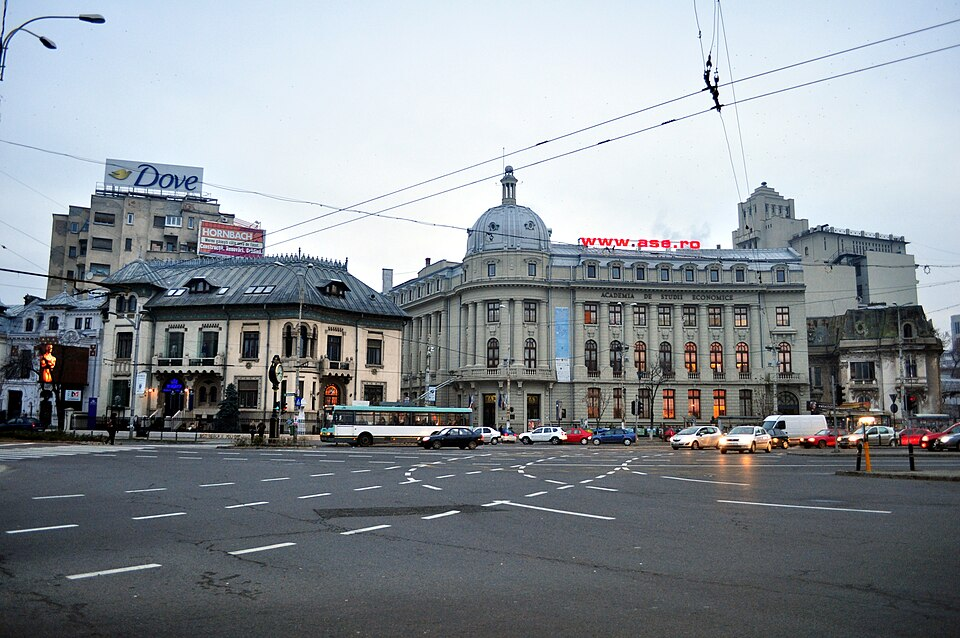
\includegraphics[height=0.40\textheight]{ch0_ase_2014.jpg}\\[1mm]
\imgcap{Bucharest University of Economic Studies}
\imgcredit{https://commons.wikimedia.org/wiki/File:Bucharest_-_Academie_de_Studii_Economice_01.jpg}{Photo: Joe Mabel (2014); CC BY 3.0; Wikimedia Commons}
\end{column}
\end{columns}
\end{frame}

\begin{frame}{Learning outcomes}
\itemsize{\small}
\begin{itemize}
    \item Place every chapter on the map of methods and state its key idea, key formula and replication result
    \item Choose the right tool for a research question about dependent data
    \item Plan a project from the question to the report, with a pre-registration and a power calculation for the evaluation
    \item Replicate a landmark paper, explain a failed replication and make every number reproducible
    \item Recognise data snooping, leakage, look-ahead, p-hacking and overclaiming in your own work
    \item Prepare the individual oral defence and document the use of AI tools
\end{itemize}
\end{frame}

\begin{frame}{Assessment at a glance}
\itemsize{\small}
\begin{center}
\footnotesize
\begin{tabular}{>{\raggedright\arraybackslash}p{3.6cm}>{\raggedright\arraybackslash}p{1.4cm}>{\raggedright\arraybackslash}p{1.6cm}>{\raggedright\arraybackslash}p{6.6cm}}
\toprule
\textbf{Component} & \textbf{Weight} & \textbf{Who} & \textbf{Content} \\
\midrule
Proposal and pre-registration & 5\% & team & question, paper to replicate, data, evaluation design fixed before estimation \\
Replication and extension & 15\% & team & repository, report in the form of a paper, AI\_USE.md, AI\_ERRORS.md \\
Oral defence & 50\% & each student & about 15 minutes: 5 minutes presenting one's own contribution, 10 minutes of questions on the code, the method and the results \\
Chapter quizzes & 20\% & each student & online, first attempt graded \\
Attendance & 10\% & each student & lectures and seminars \\
\bottomrule
\end{tabular}
\end{center}
\begin{itemize}
    \item Teams of at most three students; the project can be written and defended in Romanian or in English
    \item Grades of team members can differ: half of the final grade is individual
\end{itemize}
\end{frame}


%=============================================================================
\section{The course map}
%=============================================================================

\begin{frame}{The course map}
\itemsize{\footnotesize}
\hyphenpenalty=10000\relax
\begin{center}
\begin{tikzpicture}[font=\tiny, box/.style={draw=MainBlue, rounded corners=2pt, fill=MainBlue!6, align=center, text width=2.75cm, minimum height=0.55cm, inner sep=2pt},
  base/.style={box, draw=Forest, fill=Forest!8, text width=3.6cm}, proj/.style={box, draw=IDAred, fill=IDAred!8, text width=3.2cm, font=\scriptsize},
  head/.style={font=\scriptsize\bfseries, text=MainBlue, align=center, text width=2.9cm}, ar/.style={-{Stealth[length=1.6mm]}, MainBlue!70, thick}]
\node[base] (c0) at (-2.1,2.75) {\textbf{0} Inference for dependent data};
\node[base] (c1) at (2.1,2.75) {\textbf{1} Forecast evaluation and combination};
\node[head] (h1) at (-4.95,1.85) {Structure and identification};
\node[head] (h2) at (-1.65,1.85) {Latent states};
\node[head] (h3) at (1.65,1.85) {Volatility and risk};
\node[head] (h4) at (4.95,1.85) {Frequency and learning};
\node[box] (c2) at (-4.95,1.2) {\textbf{2} Breaks and nonlinear models};
\node[box] (c3) at (-4.95,0.5) {\textbf{3} SVAR and local projections};
\node[box] (c4) at (-4.95,-0.2) {\textbf{4} Cointegration, VECM, ARDL, panels};
\node[box] (c5) at (-4.95,-0.9) {\textbf{5} BVAR, factors, nowcasting};
\node[box] (c6) at (-1.65,1.2) {\textbf{6} State space and Bayesian filtering};
\node[box] (c7) at (-1.65,0.5) {\textbf{7} Regime switching};
\node[box] (c8) at (1.65,1.2) {\textbf{8} Realised measures, HAR, MGARCH};
\node[box] (c9) at (1.65,0.5) {\textbf{9} VaR, ES and backtesting};
\node[box] (c10) at (1.65,-0.2) {\textbf{10} Long memory and rough volatility};
\node[box] (c11) at (4.95,1.2) {\textbf{11} Spectral and wavelet analysis};
\node[box] (c12) at (4.95,0.5) {\textbf{12} Machine and deep learning};
\node[box] (c13) at (4.95,-0.2) {\textbf{13} Foundation models, conformal};
\node[box] (c14) at (-3.3,-1.95) {\textbf{14} Causal inference for time series};
\node[box] (c16) at (0,-1.95) {\textbf{16} Explosive roots and bubbles (self-study)};
\node[proj] (c15) at (3.6,-1.95) {\textbf{15} Project: replication, extension, defence};
\draw[ar] (c0.south) -- (h1.north); \draw[ar] (c0.south) -- (h2.north); \draw[ar] (c1.south) -- (h3.north); \draw[ar] (c1.south) -- (h4.north);
\draw[ar] (c0) -- (c1);
\draw[ar] (c16) -- (c15); \draw[ar] (c14.north east) to[out=20, in=160] (c15.north west);
\draw[ar, dashed] (c5.south) to[out=-90, in=150] (c14.north west);
\draw[ar, dashed] (c13.south) to[out=-90, in=60] (c15.north);
\end{tikzpicture}
\end{center}
\begin{itemize}
    \item \atschlink{https://danpele.github.io/Advanced-Time-Series/EN/Courses/chapter0_refresher_inference.pdf}{Chapters 0} and \atschlink{https://danpele.github.io/Advanced-Time-Series/EN/Courses/chapter1_forecast_evaluation.pdf}{1} are used everywhere: inference for dependent data and honest out-of-sample evaluation
    \item Every chapter feeds the project: one landmark paper to replicate and one extension
\end{itemize}
\end{frame}

\begin{frame}{Five questions for every analysis}
\itemsize{\footnotesize}
\begin{itemize}
    \item \textbf{Target}: which functional is forecast or estimated (mean, quantile, distribution, causal effect)?
    \begin{itemize}
        \item the loss or score must be consistent for it (\atschlink{https://danpele.github.io/Advanced-Time-Series/EN/Courses/chapter1_forecast_evaluation.pdf}{Chapters 1} and \atschlink{https://danpele.github.io/Advanced-Time-Series/EN/Courses/chapter9_var_es_backtesting.pdf}{9})
    \end{itemize}
    \item \textbf{Dependence}: which standard errors are valid with autocorrelation, heteroskedasticity and persistence?
    \begin{itemize}
        \item HAC with fixed-$b$ or EWC, block bootstrap, Monte Carlo size at your persistence (\atschlink{https://danpele.github.io/Advanced-Time-Series/EN/Courses/chapter0_refresher_inference.pdf}{Chapter 0})
    \end{itemize}
    \item \textbf{Identification}: what assumption turns a correlation into the claim you make?
    \begin{itemize}
        \item ordering, sign, instrument, donor pool, regime labels (\atschlink{https://danpele.github.io/Advanced-Time-Series/EN/Courses/chapter3_structural_var_local_projections.pdf}{Chapters 3}, \atschlink{https://danpele.github.io/Advanced-Time-Series/EN/Courses/chapter7_regime_switching_models.pdf}{7}, \atschlink{https://danpele.github.io/Advanced-Time-Series/EN/Courses/chapter14_causal_inference_time_series.pdf}{14})
    \end{itemize}
    \item \textbf{Evaluation}: is the design fixed before the results, in real time, with a test that fits?
    \begin{itemize}
        \item DM--HLN, Clark--West for nested models, MCS and SPA for many
    \end{itemize}
    \item \textbf{Robustness}: does the conclusion survive the forks of the analysis?
    \begin{itemize}
        \item every chapter ends with a mini-case that varies the specification
    \end{itemize}
\end{itemize}
\end{frame}

\begin{frame}{Three threads across the course}
\itemsize{\small}
\begin{itemize}
    \item \textbf{Inference under dependence}
    \begin{itemize}
        \item long-run variance $\Omega = 2\pi f(0)$ (\atschlink{https://danpele.github.io/Advanced-Time-Series/EN/Courses/chapter0_refresher_inference.pdf}{Chapter 0}) reappears in DM tests (\atschlink{https://danpele.github.io/Advanced-Time-Series/EN/Courses/chapter1_forecast_evaluation.pdf}{Chapter 1}), local projections (\atschlink{https://danpele.github.io/Advanced-Time-Series/EN/Courses/chapter3_structural_var_local_projections.pdf}{Chapter 3}), cumulative effects (\atschlink{https://danpele.github.io/Advanced-Time-Series/EN/Courses/chapter14_causal_inference_time_series.pdf}{Chapter 14})
        \item non-standard limits: sup-tests for breaks, Johansen trace, regime tests, GSADF; critical values from the right distribution
    \end{itemize}
    \item \textbf{Honest out-of-sample evaluation}
    \begin{itemize}
        \item proper scores and consistent losses, real-time data, blocked validation, evaluation after model release (\atschlink{https://danpele.github.io/Advanced-Time-Series/EN/Courses/chapter1_forecast_evaluation.pdf}{Chapters 1}, \atschlink{https://danpele.github.io/Advanced-Time-Series/EN/Courses/chapter9_var_es_backtesting.pdf}{9}, \atschlink{https://danpele.github.io/Advanced-Time-Series/EN/Courses/chapter12_machine_learning_deep_learning.pdf}{12}, \atschlink{https://danpele.github.io/Advanced-Time-Series/EN/Courses/chapter13_foundation_models_conformal.pdf}{13})
    \end{itemize}
    \item \textbf{Identification and replication}
    \begin{itemize}
        \item structural shocks, latent states and causal effects are model-dependent; landmark results were replicated on today's data, and some did not survive
    \end{itemize}
\end{itemize}
\end{frame}


%=============================================================================
\section{Chapter recaps}
%=============================================================================

\begin{frame}{\atschlinkt{https://danpele.github.io/Advanced-Time-Series/EN/Courses/chapter0_refresher_inference.pdf}{Chapter 0}: Inference for dependent data}
\itemsize{\footnotesize}
\begin{itemize}
    \item \textbf{Key ideas}
    \begin{itemize}
        \item The precision of a mean or a slope is governed by the long-run variance, not by $\gamma_0$
        \item HAC with fixed-$b$ or EWC critical values; block bootstraps resample dependence, the wild bootstrap does not
    \end{itemize}
    \item \textbf{Key formula}
    \begin{itemize}
        \item $\Omega = \gamma_0 + 2\sum_{j\ge1}\gamma_j = 2\pi f(0)$; $\hat\Omega_{NW} = \hat\Gamma_0 + \sum_{j=1}^{L}\big(1 - \frac{j}{L+1}\big)(\hat\Gamma_j + \hat\Gamma_j')$
    \end{itemize}
    \item \textbf{Replication}
    \begin{itemize}
        \item \refEH: slope 0.52 with classical $t$ = 4.72, but fixed-$b$ $t$ = 2.04 below its critical value 2.18; 1.12 before 1989, 0.15 afterwards: \textbf{partly replicated}
        \item \refWhite{} on 50 moving-average rules for the BET: naive $p$ = 0.006, Reality Check $p$ = 0.06
    \end{itemize}
    \item \textbf{Common mistakes}
    \begin{itemize}
        \item i.i.d.\ standard errors: the naive test rejects 68.1\% of true nulls at $\phi = 0.9$, $T = 100$, and still 66.2\% at $T = 400$
        \item the best of many specifications reported without a search-adjusted $p$-value
    \end{itemize}
\end{itemize}
\end{frame}

\begin{frame}{\atschlinkt{https://danpele.github.io/Advanced-Time-Series/EN/Courses/chapter1_forecast_evaluation.pdf}{Chapter 1}: Forecast evaluation and combination}
\itemsize{\footnotesize}
\begin{itemize}
    \item \textbf{Key ideas}
    \begin{itemize}
        \item Choose the loss or score first: it defines the target (mean, median, quantile, distribution)
        \item Calibration with PIT, ranking with proper scores; DM--HLN, Clark--West for nested models, SPA and MCS for many
    \end{itemize}
    \item \textbf{Key formula}
    \begin{itemize}
        \item $\mathrm{DM} = \bar d/\sqrt{\hat\Omega_d/P}$, $\mathrm{DM}^* = \mathrm{DM}\sqrt{(P + 1 - 2h + h(h - 1)/P)/P}$ against $t_{P-1}$
    \end{itemize}
    \item \textbf{Replication}
    \begin{itemize}
        \item \refMR{} on EUR/RON: AR(1) RMSE 1.055 times the random walk, drift 1.006 (Clark--West $p$ = 0.145): \textbf{replicated}
        \item \refGKMT{} on the SPF: median 0.999, previous best 1.099 (HLN $p$ = 0.007); \refAO: ratio 1.75 but $p$ = 0.248
    \end{itemize}
    \item \textbf{Common mistakes}
    \begin{itemize}
        \item plain DM with few multi-step forecasts: size 43.6\% at $h = 8$, $P = 16$ (HLN: 14.6\%)
        \item DM on nested models; estimated combination weights for similar forecasts
    \end{itemize}
\end{itemize}
\end{frame}

\begin{frame}{\atschlinkt{https://danpele.github.io/Advanced-Time-Series/EN/Courses/chapter2_structural_breaks_nonlinear_models.pdf}{Chapter 2}: Structural breaks and nonlinear models}
\itemsize{\footnotesize}
\begin{itemize}
    \item \textbf{Key ideas}
    \begin{itemize}
        \item A break date chosen from the data is a nuisance parameter: sup, exp and ave tests with their own critical values
        \item Breaks and nonlinearity mimic each other: test one allowing for the other
    \end{itemize}
    \item \textbf{Key formula}
    \begin{itemize}
        \item $\sup_{\pi}W_T(\pi) \Rightarrow \sup_\pi \|B_p(\pi) - \pi B_p(1)\|^2/[\pi(1 - \pi)]$; TAR: $y_t = \phi_1'x_t\mathbf 1\{q_{t-d} \le \gamma\} + \phi_2'x_t\mathbf 1\{q_{t-d} > \gamma\} + \varepsilon_t$
    \end{itemize}
    \item \textbf{Replication}
    \begin{itemize}
        \item \refMPQ: break in 1984Q1, sup-$W$ = 52.5; on the sample to 2026 only 10.7; \refBP: 3 breaks at the published dates
        \item \refHanB: $\hat\gamma$ = 0.261 (paper 0.302); \refTPS: Monte Carlo $p$ = 0.165 (paper 0.002): \textbf{not replicated}
    \end{itemize}
    \item \textbf{Common mistakes}
    \begin{itemize}
        \item Chow test at a data-chosen date: size 33--40\%; the sup critical value is 8.65, not 3.84
        \item in-sample nonlinearity read as a forecasting gain
    \end{itemize}
\end{itemize}
\end{frame}

\begin{frame}{\atschlinkt{https://danpele.github.io/Advanced-Time-Series/EN/Courses/chapter3_structural_var_local_projections.pdf}{Chapter 3}: Structural VAR and local projections}
\itemsize{\footnotesize}
\begin{itemize}
    \item \textbf{Key ideas}
    \begin{itemize}
        \item A structural VAR is a reduced form plus an identifying assumption; the assumption is the economics
        \item Zeros, signs, narratives, heteroskedasticity and instruments buy identification with different assumptions; LP and VAR estimate the same responses
    \end{itemize}
    \item \textbf{Key formula}
    \begin{itemize}
        \item $u_t = B_0\varepsilon_t$, $\Theta_h = \Phi_hB_0$; proxy: $\E(u_tz_t) = \alpha b_1$; LP: $y_{t+h} = \mu_h + \beta_hx_t + \gamma_h'w_t + \xi_{t+h}$
    \end{itemize}
    \item \textbf{Replication}
    \begin{itemize}
        \item \refCEE: industrial production trough \ensuremath{-}0.27\% after 21 months, with the price puzzle; \refGK: $F$ = 17.7, excess bond premium +0.14: \textbf{replicated}
        \item \refKil: oil-price variance at 60 months: supply 1\%, aggregate demand 64\%, oil-specific demand 35\%
    \end{itemize}
    \item \textbf{Common mistakes}
    \begin{itemize}
        \item a recursive ordering read as a fact; the wild bootstrap for a proxy SVAR (use the moving-block bootstrap)
        \item a short VAR at long horizons: bias 0.71 at $h = 8$ against 0.07 for LP, at a higher variance
    \end{itemize}
\end{itemize}
\end{frame}

\begin{frame}{\atschlinkt{https://danpele.github.io/Advanced-Time-Series/EN/Courses/chapter4_cointegration_vecm_ardl_panel.pdf}{Chapter 4}: Cointegration: VECM, ARDL and panel data}
\itemsize{\footnotesize}
\begin{itemize}
    \item \textbf{Key ideas}
    \begin{itemize}
        \item Johansen is reduced-rank regression; the rank test is non-standard, depends on the deterministic case and over-rejects in small samples
        \item Given the rank, tests on $\beta$ and $\alpha$ are $\chi^2$; ARDL is a conditional VECM; panels need cross-section dependence first
    \end{itemize}
    \item \textbf{Key formula}
    \begin{itemize}
        \item $\Delta y_t = \alpha\beta'y_{t-1} + \sum_{i=1}^{p-1}\Gamma_i\Delta y_{t-i} + \Phi D_t + \varepsilon_t$, $LR_{tr}(r) = -T\sum_{i>r}\ln(1 - \hat\lambda_i)$
    \end{itemize}
    \item \textbf{Replication}
    \begin{itemize}
        \item \refKPSW: two cointegrating relations, but the great ratios rejected (LR 16.6, $p$ $<$0.001): \textbf{partly replicated}
        \item \refPSS{} on EU-27 consumption: income elasticity 0.69, Hausman $p$ = 0.300; the inflation effect is not robust
    \end{itemize}
    \item \textbf{Common mistakes}
    \begin{itemize}
        \item asymptotic critical values at $T = 50$: size 18.2\% against 4.8\% for the wild bootstrap
        \item the rank read as a measurement: Romanian pass-through, wild bootstrap $p$ = 0.647 with four lags
    \end{itemize}
\end{itemize}
\end{frame}

\begin{frame}{\atschlinkt{https://danpele.github.io/Advanced-Time-Series/EN/Courses/chapter5_bvar_factor_models_nowcasting.pdf}{Chapter 5}: Bayesian VAR, factor models and nowcasting}
\itemsize{\footnotesize}
\begin{itemize}
    \item \textbf{Key ideas}
    \begin{itemize}
        \item Many series and few observations: shrink (priors) or compress (factors); bigger systems need tighter priors
        \item Nowcasting is Kalman filtering with a ragged edge; every revision is a sum of news
    \end{itemize}
    \item \textbf{Key formula}
    \begin{itemize}
        \item Minnesota: $\Var[(A_l)_{ij}] = \lambda^2/l^2$ if $j = i$, $\vartheta\lambda^2\sigma_i^2/(l^2\sigma_j^2)$ otherwise
    \end{itemize}
    \item \textbf{Replication}
    \begin{itemize}
        \item \refBGR, employment, $h = 1$: 1.06, 0.54, 0.50 for small, medium, large (paper 1.14, 0.54, 0.46): \textbf{replicated} for 1971--2003
        \item \refSW: industrial production, $h = 12$: 0.58 in 1970--1998, but 1.07 in 1999--2019: the gain vanishes
    \end{itemize}
    \item \textbf{Common mistakes}
    \begin{itemize}
        \item a homoskedastic BVAR through 2020: relative MSFE 500.06 at 12 months
        \item ``better nowcasts'' from a lower RMSE without a test: Romanian GDP, DM $t$ = \ensuremath{-}0.30, $p$ = 0.76
    \end{itemize}
\end{itemize}
\end{frame}

\begin{frame}{\atschlinkt{https://danpele.github.io/Advanced-Time-Series/EN/Courses/chapter6_state_space_models_bayesian_filtering.pdf}{Chapter 6}: State space models and Bayesian filtering}
\itemsize{\footnotesize}
\begin{itemize}
    \item \textbf{Key ideas}
    \begin{itemize}
        \item The Kalman filter is Gaussian conditioning applied recursively; smoother, likelihood and simulation smoother follow from it
        \item Initialise nonstationary states exactly; stochastic volatility is not GARCH; latent quantities come with model-dependent bands
    \end{itemize}
    \item \textbf{Key formula}
    \begin{itemize}
        \item $v_t = y_t - Z_ta_t$, $F_t = Z_tP_tZ_t' + H_t$, $K_t = T_tP_tZ_t'F_t^{-1}$, $a_{t+1} = T_ta_t + K_tv_t$
    \end{itemize}
    \item \textbf{Replication}
    \begin{itemize}
        \item \refMNZ{} on today's GDP vintage: $\hat\rho$ = \ensuremath{-}0.927, correlation with the Beveridge--Nelson cycle 0.999; cycle s.d.\ 2.20 (UC0) against 0.52: \textbf{replicated}
        \item Stochastic volatility beats GARCH on the S\&P 500 by 88.5 log-likelihood points
    \end{itemize}
    \item \textbf{Common mistakes}
    \begin{itemize}
        \item a zero variance estimate read as a constant level: 64\% of estimates are exactly zero when the true variance is zero (pile-up)
        \item a ``big kappa'' initialisation; an output gap without its band
    \end{itemize}
\end{itemize}
\end{frame}

\begin{frame}{\atschlinkt{https://danpele.github.io/Advanced-Time-Series/EN/Courses/chapter7_regime_switching_models.pdf}{Chapter 7}: Regime-switching models}
\itemsize{\footnotesize}
\begin{itemize}
    \item \textbf{Key ideas}
    \begin{itemize}
        \item The Hamilton filter and the Kim smoother are exact recursions for a discrete latent state; EM finds local and degenerate maxima
        \item The number of regimes is a non-standard testing problem; regimes, breaks and long memory are observationally close
    \end{itemize}
    \item \textbf{Key formula}
    \begin{itemize}
        \item $\hat\xi_{t|t} = \hat\xi_{t|t-1}\odot\eta_t/\mathbf 1'(\hat\xi_{t|t-1}\odot\eta_t)$, $\hat\xi_{t+1|t} = \mathbf P'\hat\xi_{t|t}$, $\E D_i = 1/(1 - p_{ii})$
    \end{itemize}
    \item \textbf{Replication}
    \begin{itemize}
        \item \refHam{} on his data: log-likelihood \ensuremath{-}181.26 with two implementations, QPS 0.179: \textbf{replicated exactly}
        \item On today's data the low regime becomes sharp falls: 2008Q4 probability 0.95, 2001 at most 0.01
    \end{itemize}
    \item \textbf{Common mistakes}
    \begin{itemize}
        \item $\chi^2$ critical values for the number of regimes: LR 71.7, bootstrap 95\% quantile 12.32, not 5.99
        \item statistical regimes read as economic regimes; smoothed probabilities used to judge real-time dating
    \end{itemize}
\end{itemize}
\end{frame}

\begin{frame}{\atschlinkt{https://danpele.github.io/Advanced-Time-Series/EN/Courses/chapter8_advanced_volatility.pdf}{Chapter 8}: Advanced volatility modelling}
\itemsize{\footnotesize}
\begin{itemize}
    \item \textbf{Key ideas}
    \begin{itemize}
        \item Gaussian QML needs only the variance equation; with fat tails, use sandwich standard errors
        \item Realised measures make volatility observable with a known error; HAR, HARQ and Realized GARCH win one day ahead
    \end{itemize}
    \item \textbf{Key formula}
    \begin{itemize}
        \item HARQ: $\mathrm{RV}_{t+1} = \beta_0 + (\beta_d + \beta_{dQ}\sqrt{\mathrm{RQ}_t})\mathrm{RV}_t + \beta_w\mathrm{RV}^{(w)}_t + \beta_m\mathrm{RV}^{(m)}_t + u_{t+1}$
    \end{itemize}
    \item \textbf{Replication}
    \begin{itemize}
        \item \refBPQ{} on crypto: QLIKE relative to HAR 0.946 (Bitcoin), 0.921 (Ether); \refEGS: industrial production $t$ = \ensuremath{-}1.56, only the realised-variance driver works ($t$ = 3.86)
        \item \refELW: GMV volatility 18.33 (DCC-NL) against 18.35 (DCC): the gain does not appear here: \textbf{not replicated}
    \end{itemize}
    \item \textbf{Common mistakes}
    \begin{itemize}
        \item Hessian standard errors with Student-$t(5)$ errors: coverage 73.0\% against 91.7\% for the sandwich
        \item non-robust losses (MAE, MSE on logs) with a noisy volatility proxy
    \end{itemize}
\end{itemize}
\end{frame}

\begin{frame}{\atschlinkt{https://danpele.github.io/Advanced-Time-Series/EN/Courses/chapter9_var_es_backtesting.pdf}{Chapter 9}: VaR, ES and backtesting}
\itemsize{\footnotesize}
\begin{itemize}
    \item \textbf{Key ideas}
    \begin{itemize}
        \item A risk forecast is a point forecast of a functional: judge it with a consistent loss; VaR is elicitable, ES only jointly with VaR
        \item Backtests are moment tests with estimation risk; comparisons need DM, MCS and Murphy diagrams
    \end{itemize}
    \item \textbf{Key formula}
    \begin{itemize}
        \item $L_{\mathrm{FZ0}}(y, v, e; \alpha) = -\frac{1}{\alpha e}\mathbf 1\{y \le v\}(v - y) + \frac{v}{e} + \ln(-e) - 1$; $\mathrm{VaR}_\alpha = -q_\alpha$
    \end{itemize}
    \item \textbf{Replication}
    \begin{itemize}
        \item \refPZC: GAS-1F loss 0.853 (paper 0.853): the ranking \textbf{replicates}; its goodness-of-fit $p$-values 0.001 and 0.037 (paper 0.242 and 0.313) \textbf{do not}
        \item \refEM{} out of sample: only IG passes the DQ test ($p$ = 0.891; SAV 0.025)
    \end{itemize}
    \item \textbf{Common mistakes}
    \begin{itemize}
        \item ranking ES forecasts alone; Normal VaR 1\% with a hit rate of 2.2\%
        \item the $\sqrt{h}$ rule under volatility clustering; ``the best ES model'' instead of the MCS
    \end{itemize}
\end{itemize}
\end{frame}

\begin{frame}{\atschlinkt{https://danpele.github.io/Advanced-Time-Series/EN/Courses/chapter10_long_memory_rough_volatility.pdf}{Chapter 10}: Long memory and rough volatility}
\itemsize{\footnotesize}
\begin{itemize}
    \item \textbf{Key ideas}
    \begin{itemize}
        \item Long memory is a pole at frequency zero; estimate $d$ by (exact) local Whittle and report $\hat d(m)$ across bandwidths
        \item Volatility is persistent over months and rough over days ($H \approx 0.1$); level shifts mimic long memory
    \end{itemize}
    \item \textbf{Key formula}
    \begin{itemize}
        \item $f(\lambda) \sim c_f\lambda^{-2d}$, $\gamma(k) \sim c_\gamma k^{2d-1}$; $\E|\ln\sigma_{t+\Delta} - \ln\sigma_t|^q \propto \Delta^{qH}$
    \end{itemize}
    \item \textbf{Replication}
    \begin{itemize}
        \item \refGJR{} on the S\&P 500: $\hat H$ = 0.149 (0.140 and 0.155 in two halves): \textbf{replicated}; \refQu: $W$ = 0.66, the memory of realised variance survives
        \item Rough forecasting gain over HAR at 5 days: QLIKE ratio 0.964, $p$ = 0.07: small and horizon-dependent
    \end{itemize}
    \item \textbf{Common mistakes}
    \begin{itemize}
        \item one bandwidth, one $\hat d$; ``short memory because $H < 1/2$'' (roughness and persistence are different properties)
    \end{itemize}
\end{itemize}
\end{frame}

\begin{frame}{\atschlinkt{https://danpele.github.io/Advanced-Time-Series/EN/Courses/chapter11_spectral_wavelet_analysis.pdf}{Chapter 11}: Spectral and wavelet analysis}
\itemsize{\footnotesize}
\begin{itemize}
    \item \textbf{Key ideas}
    \begin{itemize}
        \item The spectrum decomposes variance by frequency; filters act on it through their squared gain; multitaper gives low leakage and honest bands
        \item Wavelets localise variance and co-movement in time and scale; significance needs Monte Carlo and areawise thinking
    \end{itemize}
    \item \textbf{Key formula}
    \begin{itemize}
        \item HP cycle gain $G(\omega) = \dfrac{4\lambda(1 - \cos\omega)^2}{1 + 4\lambda(1 - \cos\omega)^2}$; coherence $\kappa^2(\omega) = |f_{xy}|^2/(f_xf_y)$
    \end{itemize}
    \item \textbf{Replication}
    \begin{itemize}
        \item \refCN: HP applied to a random walk peaks at 30.1 quarters (7.5 years; simulation 28.6): \textbf{replicated}
        \item \refHamB{} on Romanian GDP: the real-time HP gap correlates 0.57 with the final one and has the wrong sign in 38\% of quarters
    \end{itemize}
    \item \textbf{Common mistakes}
    \begin{itemize}
        \item every wavelet-coherence island read as contagion: BET--DAX 23\% significant area against a null 95\% quantile of 7.7\%
        \item pointwise tests across frequencies read as a joint test
    \end{itemize}
\end{itemize}
\end{frame}

\begin{frame}{\atschlinkt{https://danpele.github.io/Advanced-Time-Series/EN/Courses/chapter12_machine_learning_deep_learning.pdf}{Chapter 12}: Machine learning and deep learning}
\itemsize{\footnotesize}
\begin{itemize}
    \item \textbf{Key ideas}
    \begin{itemize}
        \item Validation must respect dependence: K-fold only for well-specified autoregressions; otherwise block, purge and keep a final test period
        \item Trees and networks rarely beat strong structured baselines alone; global models pool series; seeds and searches are hidden multiple testing
    \end{itemize}
    \item \textbf{Key formula}
    \begin{itemize}
        \item $\mathrm{OWA} = \frac12\big(\mathrm{sMAPE}/\mathrm{sMAPE}_{\mathrm{Naive2}} + \mathrm{MASE}/\mathrm{MASE}_{\mathrm{Naive2}}\big)$; $\mathrm{Att}(Q, K, V) = \mathrm{softmax}(QK'/\sqrt{d_k})V$
    \end{itemize}
    \item \textbf{Replication}
    \begin{itemize}
        \item \refBHK: 5-fold CV error 0.094 against 0.137 out of sample: \textbf{replicated}
        \item \refZeng{} and \refNie{} on Romanian load, $H = 96$: point-token Transformer 0.258, DLinear 0.257, patches 0.226: both papers \textbf{replicate}
    \end{itemize}
    \item \textbf{Common mistakes}
    \begin{itemize}
        \item random K-fold with autocorrelated residuals: validation-to-test error ratio 0.34 (leakage)
        \item attention weights read as importance; the best of many seeds reported as the model
    \end{itemize}
\end{itemize}
\end{frame}

\begin{frame}{\atschlinkt{https://danpele.github.io/Advanced-Time-Series/EN/Courses/chapter13_foundation_models_conformal.pdf}{Chapter 13}: Foundation models and conformal prediction}
\itemsize{\footnotesize}
\begin{itemize}
    \item \textbf{Key ideas}
    \begin{itemize}
        \item Foundation models amortise estimation over a corpus; evaluate after release, pool across series, correct for multiplicity
        \item Conformal prediction gives finite-sample marginal coverage under exchangeability; under dependence, ACI restores long-run coverage
    \end{itemize}
    \item \textbf{Key formula}
    \begin{itemize}
        \item $\hat q = S_{(\lceil(n + 1)(1 - \alpha)\rceil)}$; ACI: $\alpha_{t+1} = \alpha_t + \gamma(\alpha - \mathrm{err}_t)$
    \end{itemize}
    \item \textbf{Replication}
    \begin{itemize}
        \item \refGC{} on the S\&P 500 (target 0.90): static coverage 0.918, ACI 0.901; \refRPC: raw quantiles 0.883, CQR 0.915: \textbf{replicated}
        \item Romanian load: Chronos-2 MAE 0.210 against 0.221 for the expert ARX
    \end{itemize}
    \item \textbf{Common mistakes}
    \begin{itemize}
        \item cherry-picked countries: Chronos-2 better in 23 of 27 inflation series, significant in 0 after Holm
        \item evaluation windows before the model release; conditional coverage claimed instead of tested
    \end{itemize}
\end{itemize}
\end{frame}

\begin{frame}{\atschlinkt{https://danpele.github.io/Advanced-Time-Series/EN/Courses/chapter14_causal_inference_time_series.pdf}{Chapter 14}: Causal inference for time series}
\itemsize{\footnotesize}
\begin{itemize}
    \item \textbf{Key ideas}
    \begin{itemize}
        \item Granger causality and its relatives (TE, PCMCI, CCM) describe predictive structure; causal claims need assumptions about the assignment
        \item Synthetic control uses other units: placebos are the inference, a long pre-period fit is the justification
    \end{itemize}
    \item \textbf{Key formula}
    \begin{itemize}
        \item $w^* = \arg\min_w(X_1 - X_0w)'V(X_1 - X_0w)$, $w_j \ge 0$, $\sum_jw_j = 1$; placebo $p = \#\{j: r_j \ge r_1\}/(J + 1)$
    \end{itemize}
    \item \textbf{Replication}
    \begin{itemize}
        \item \refADH: West German GDP per capita 1588 USD a year (5.6\%) below its synthetic control, placebo $p$ = 0.059: \textbf{replicated}
        \item \refBMSS{} on revised data: gap $-$1.5\% in 2018Q4 (paper $-$2.4\%), UK rank 11 of 24: \textbf{not replicated in strength}
    \end{itemize}
    \item \textbf{Common mistakes}
    \begin{itemize}
        \item Granger causality read as causation; a common driver produces it
        \item synthetic control outside the convex hull: classic SC gives 4.18 pp for Romania, the robust estimators 2.7--2.8 pp
    \end{itemize}
\end{itemize}
\end{frame}

\begin{frame}{\atschlinkt{https://danpele.github.io/Advanced-Time-Series/EN/Courses/chapter16_explosive_roots_bubbles.pdf}{Chapter 16}: Explosive roots and bubbles (self-study)}
\itemsize{\footnotesize}
\begin{itemize}
    \item \textbf{Key ideas}
    \begin{itemize}
        \item A rational bubble is an explosive component; periodically collapsing bubbles hide from whole-sample tests
        \item Critical values must match the design: wild bootstrap under changing volatility, family-wise control for date-stamping
    \end{itemize}
    \item \textbf{Key formula}
    \begin{itemize}
        \item $\mathrm{BSADF}_{r_2} = \sup_{r_1}\mathrm{ADF}_{r_1}^{r_2}$, $\mathrm{GSADF} = \sup_{r_2}\mathrm{BSADF}_{r_2}$; bubble: $\E_tB_{t+1} = (1 + r)B_t$
    \end{itemize}
    \item \textbf{Replication}
    \begin{itemize}
        \item \refPY: US price-to-rent GSADF 5.75 against the wild critical value 4.47: \textbf{replicated}
        \item \refPWY{} Nasdaq: 2.92 rejects with Monte Carlo (2.28) but not with the wild bootstrap (3.22); \refPSY{} S\&P 500: 2.19 below both: \textbf{not replicated}
    \end{itemize}
    \item \textbf{Common mistakes}
    \begin{itemize}
        \item Monte Carlo critical values after a volatility shift: size 33.8\% (wild bootstrap 3.2\%)
        \item pointwise date-stamping read as a 5\% test: false episodes in 32.5\% of no-bubble paths
    \end{itemize}
\end{itemize}
\end{frame}

\begin{frame}{Recap: chapter recaps}
\itemsize{\small}
\begin{itemize}
    \item Most landmark results replicate in direction on today's data; their strength and their tests often do not
    \item The same mistakes recur: i.i.d.\ inference on dependent data, the wrong critical values, a search reported as one test
    \item Every chapter offers a replication and an extension for the project (\atsapplink{atsapp1}{atssrc1}{Appendix})
\end{itemize}
\end{frame}


%=============================================================================
\section{The methods toolbox}
%=============================================================================

\begin{frame}{Which tool for which question (1/3): inference and evaluation}
\itemsize{\small}
\begin{center}
\scriptsize
\begin{tabular}{>{\raggedright\arraybackslash}p{5.6cm}>{\raggedright\arraybackslash}p{6.2cm}>{\raggedright\arraybackslash}p{0.8cm}}
\toprule
\textbf{Research question} & \textbf{Tool} & \textbf{Ch.} \\
\midrule
Is a mean, a slope or a predictive coefficient different from zero? & HAC with fixed-$b$ or EWC; block bootstrap; Monte Carlo size check & 0 \\
Does one of many rules or models beat a benchmark? & Reality Check, SPA, StepM; MCS & 0, 1 \\
Is forecast A more accurate than forecast B? & DM--HLN with HAC; Clark--West if nested; Giacomini--White for methods & 1 \\
Is a density or interval forecast calibrated? & PIT, Berkowitz; coverage and independence tests; CRPS, log score & 1, 13 \\
Is a VaR or (VaR, ES) forecast adequate, and which is best? & Kupiec, Christoffersen, DQ; FZ0 loss, DM, MCS, Murphy diagrams & 9 \\
Do my intervals keep their coverage under dependence? & split conformal, CQR, ACI, conformal PID; coverage by regime & 13 \\
\bottomrule
\end{tabular}
\end{center}
\end{frame}

\begin{frame}{Which tool for which question (2/3): structure and dynamics}
\itemsize{\small}
\begin{center}
\scriptsize
\begin{tabular}{>{\raggedright\arraybackslash}p{5.6cm}>{\raggedright\arraybackslash}p{6.2cm}>{\raggedright\arraybackslash}p{0.8cm}}
\toprule
\textbf{Research question} & \textbf{Tool} & \textbf{Ch.} \\
\midrule
Did the parameters change, and when? & sup/exp/ave tests, Bai--Perron, CSW monitoring, variance-break tests & 2 \\
Is the dynamics nonlinear or state-dependent? & TAR, STAR with bootstrap or LM tests; Markov switching with bootstrap LR & 2, 7 \\
What is the effect of a structural shock? & SVAR (zeros, signs, proxies), local projections, LP-IV & 3 \\
Is there a long-run equilibrium, and who adjusts? & Johansen with bootstrap; tests on $\beta$ and $\alpha$; ARDL bounds; panel CCE and PMG & 4 \\
How to forecast with many predictors or mixed frequencies? & BVAR with optimised shrinkage, factors, DFM nowcasting, MIDAS & 5 \\
What is the unobserved trend, gap or time-varying slope? & state space by ML or Gibbs, simulation smoother, UC-SV, particle filters & 6 \\
\bottomrule
\end{tabular}
\end{center}
\end{frame}

\begin{frame}{Which tool for which question (3/3): volatility, frequency, learning, causality}
\itemsize{\small}
\begin{center}
\scriptsize
\begin{tabular}{>{\raggedright\arraybackslash}p{5.6cm}>{\raggedright\arraybackslash}p{6.2cm}>{\raggedright\arraybackslash}p{0.8cm}}
\toprule
\textbf{Research question} & \textbf{Tool} & \textbf{Ch.} \\
\midrule
How to forecast volatility or a covariance matrix? & HAR, HARQ, Realized GARCH; DCC with shrinkage; QLIKE & 8 \\
Is the memory long, or is it shifts? & local Whittle $\hat d(m)$, Qu test, scaling of log volatility & 10 \\
At which frequencies do two series move together? & multitaper coherence and phase, Breitung--Candelon, wavelet coherence & 11 \\
Do flexible learners or foundation models beat the baseline? & blocked validation, strong baselines, pooled tests, Holm and BH & 12, 13 \\
Does $x$ help predict $y$, and did a policy have an effect? & conditional Granger, PCMCI; ITS, synthetic control with placebos, CausalImpact & 14 \\
Is there a bubble, and when did it start? & GSADF and BSADF with wild bootstrap, family-wise dating & 16 \\
\bottomrule
\end{tabular}
\end{center}
\end{frame}


%=============================================================================
\section{The research workflow}
%=============================================================================

\begin{frame}{The project in eight steps}
\itemsize{\small}
\begin{center}
\begin{tikzpicture}[font=\scriptsize, st/.style={draw=MainBlue, rounded corners=3pt, fill=MainBlue!6, minimum width=2.6cm, minimum height=0.8cm, align=center}, ar/.style={-{Stealth[length=1.8mm]}, MainBlue!70, thick}]
\node[st] (s0) at (0.0,0) {\textbf{1}. Question};
\node[st] (s1) at (3.2,0) {\textbf{2}. Literature};
\node[st] (s2) at (6.4,0) {\textbf{3}. Pre-registration};
\node[st] (s3) at (9.600000000000001,0) {\textbf{4}. Data};
\node[st] (s4) at (9.600000000000001,-1.5) {\textbf{5}. Replication};
\node[st] (s5) at (6.4,-1.5) {\textbf{6}. Extension};
\node[st] (s6) at (3.2,-1.5) {\textbf{7}. Robustness};
\node[st] (s7) at (0.0,-1.5) {\textbf{8}. Reporting};
\draw[ar] (s0) -- (s1); \draw[ar] (s1) -- (s2); \draw[ar] (s2) -- (s3); \draw[ar] (s3) -- (s4); \draw[ar] (s4) -- (s5); \draw[ar] (s5) -- (s6); \draw[ar] (s6) -- (s7);
\draw[decorate, decoration={brace, amplitude=4pt}, IDAred] (-1.3,0.6) -- (7.7,0.6) node[midway, above=4pt, text=IDAred] {proposal and pre-registration: 5\%};
\draw[decorate, decoration={brace, amplitude=4pt, mirror}, IDAred] (-1.3,-2.1) -- (10.9,-2.1) node[midway, below=4pt, text=IDAred] {repository, report, AI\_USE.md, AI\_ERRORS.md: 15\%; defence of every step: 50\%};
\end{tikzpicture}
\end{center}
\begin{itemize}
    \item The order matters: the evaluation design is fixed before the first estimate, the replication comes before the extension
    \item Each step leaves a trace in the repository (a file, a commit, a section of the report)
\end{itemize}
\end{frame}

\begin{frame}{Steps 1--2: the question and the literature}
\itemsize{\small}
\begin{itemize}
    \item \textbf{A good question} is narrow, falsifiable and answerable with public data
    \begin{itemize}
        \item ``Does the Meese--Rogoff result hold for EUR/RON at horizons of 1--12 months after 2015?'' rather than ``Can we forecast exchange rates?''
    \end{itemize}
    \item \textbf{The landmark paper}: one of the case studies of \atschlink{https://danpele.github.io/Advanced-Time-Series/EN/Courses/chapter0_refresher_inference.pdf}{Chapters 0}--\atschlink{https://danpele.github.io/Advanced-Time-Series/EN/Courses/chapter16_explosive_roots_bubbles.pdf}{16}, or another paper approved in advance
    \begin{itemize}
        \item identify the table or figure you will reproduce, the sample, the data source and the code, if published
    \end{itemize}
    \item \textbf{The literature}: what was found since, and what is still open
    \begin{itemize}
        \item every reference checked against its DOI; an AI-suggested reference is a hypothesis until verified \refWW
    \end{itemize}
    \item The extension answers a new question: new data (Romania, the EU, recent years), a new method from the course, or a new test
\end{itemize}
\end{frame}

\begin{frame}{Step 3: the pre-registration}
\itemsize{\small}
\begin{itemize}
    \item A pre-registration fixes the analysis before the data can influence it \refNos
    \begin{itemize}
        \item the hypotheses and the primary outcome
        \item the data: sources, vintages, sample, transformations, exclusions
        \item the evaluation: estimation and test windows, horizons, losses, tests, the benchmark
        \item the multiplicity plan: how many comparisons, which correction (Holm, MCS, SPA)
        \item the robustness rule: which variations, and what counts as a robust result
    \end{itemize}
    \item A power calculation for the evaluation: is the test sample long enough to detect the published gain? (mini-case at the end)
    \item Deviations are allowed but reported: the pre-registration is a commitment to transparency, not a prison
\end{itemize}
\end{frame}

\begin{frame}{Steps 4--6: data, replication, extension}
\itemsize{\small}
\begin{itemize}
    \item \textbf{Data}: official sources, documented once
    \begin{itemize}
        \item market data from the course repository (EODHD); FRED, Eurostat, ECB, INS, BNR online; record the download date (vintage)
        \item real-time questions need real-time data: revised data flatter forecasts (\atschlink{https://danpele.github.io/Advanced-Time-Series/EN/Courses/chapter1_forecast_evaluation.pdf}{Chapters 1} and \atschlink{https://danpele.github.io/Advanced-Time-Series/EN/Courses/chapter5_bvar_factor_models_nowcasting.pdf}{5})
    \end{itemize}
    \item \textbf{Replication}: first the original sample and specification, then today's data
    \begin{itemize}
        \item a table that puts the published numbers next to yours, with the differences explained
    \end{itemize}
    \item \textbf{Extension}: one new question, answered with the same care
    \begin{itemize}
        \item new sample, new country, new method of the course, or a stronger test of the original claim
    \end{itemize}
\end{itemize}
\end{frame}

\begin{frame}{Steps 7--8: robustness and reporting}
\itemsize{\small}
\begin{itemize}
    \item \textbf{Robustness}: show the distribution of results over reasonable choices, not the best one
    \begin{itemize}
        \item specification curve or multiverse \refSSN, \refSte: windows, lags, donor pools, losses, bandwidths
        \item 164 teams testing the same hypotheses on the same data disagree as much as the standard errors suggest \refMen
    \end{itemize}
    \item \textbf{Report} in the form of a paper: introduction, data, method, replication, extension, robustness, conclusion
    \begin{itemize}
        \item every number in the text produced by the code; figures with the course chart rules
        \item effect sizes with confidence intervals, not stars; limits stated explicitly
    \end{itemize}
    \item AI\_USE.md and AI\_ERRORS.md in the repository (section on AI in research)
\end{itemize}
\end{frame}

\begin{frame}{Recap: the research workflow}
\itemsize{\small}
\begin{itemize}
    \item Question, literature and pre-registration come before any estimate
    \item Replicate on the original sample first; extend with one new question
    \item Report the distribution over specifications and every deviation from the plan
\end{itemize}
\end{frame}


%=============================================================================
\section{Replicating a landmark paper}
%=============================================================================

\begin{frame}{Reproduction, replication, robustness}
\itemsize{\small}
\begin{itemize}
    \item \refCle{} distinguishes
    \begin{itemize}
        \item \textbf{verification}: same data, same code, same numbers (a computational check)
        \item \textbf{reproduction}: same specification and population, re-coded or with re-collected data
        \item \textbf{robustness}: a different specification, sample or population: an extension, not a failure if it differs
    \end{itemize}
    \item In economics, about half of the papers can be reproduced from the authors' files without their help \refCL; anomalies in finance often fail on extended samples \refHXZ
    \item A spreadsheet error changed a policy debate: \refHAP
    \item In the course, almost every replication was a reproduction on today's data, followed by a robustness check
\end{itemize}
\end{frame}

\begin{frame}{Scoreboard of the course replications (1/2)}
\itemsize{\small}
\begin{center}
\scriptsize
\begin{tabular}{>{\raggedright\arraybackslash}p{4.3cm}l>{\raggedright\arraybackslash}p{1.7cm}>{\raggedright\arraybackslash}p{6.2cm}}
\toprule
\textbf{Paper} & \textbf{Ch.} & \textbf{Verdict} & \textbf{What decided it} \\
\midrule
\refEH{} & 0 & partly & robust inference and a later sample remove the significance \\
\refMR, \refGKMT{} & 1 & replicated & random walk and the simple average are hard to beat \\
\refMPQ, \refBP{} & 2 & replicated & dates reproduced; the 2020 outliers weaken the extension \\
\refHanB{} & 2 & partly & threshold close, delay fragile on revised data \\
\refTPS{} & 2 & not replicated & Monte Carlo $p$-value; the price index of the paper is not published today \\
\refCEE, \refKil, \refGK{} & 3 & replicated & public replication files; same identification \\
\refKPSW{} & 4 & partly & rank reproduced, great ratios depend on the deterministic case \\
\refBGR{} & 5 & replicated & to 2003; fails after 2020 without stochastic volatility \\
\refSW{} & 5 & partly & gains vanish on 1999--2019 \\
\refMNZ, \refHam{} & 6, 7 & replicated & same data; Hamilton's dating does not survive today's sample \\
\bottomrule
\end{tabular}
\end{center}
\end{frame}

\begin{frame}{Scoreboard of the course replications (2/2)}
\itemsize{\small}
\begin{center}
\scriptsize
\begin{tabular}{>{\raggedright\arraybackslash}p{4.3cm}l>{\raggedright\arraybackslash}p{1.7cm}>{\raggedright\arraybackslash}p{6.2cm}}
\toprule
\textbf{Paper} & \textbf{Ch.} & \textbf{Verdict} & \textbf{What decided it} \\
\midrule
\refBPQ{} & 8 & replicated & in QLIKE; the ranking changes in MSE \\
\refEGS{} & 8 & partly & the sign survives, the macro effect is not significant \\
\refELW{} & 8 & not replicated & few assets relative to the sample: shrinkage has little to do \\
\refPZC{} & 9 & partly & average losses reproduced; tests on a few tail days do not \\
\refGJR, \refQu{} & 10 & replicated & scaling stable across halves and markets \\
\refCN, \refHamB{} & 11 & replicated & a property of the filter, not of the data \\
\refBHK, \refZeng{} & 12 & replicated & protocols reproduced on Romanian load \\
\refGC, \refRPC{} & 13 & replicated & finite-sample guarantees hold by construction \\
\refADH{} & 14 & replicated & public data and code; weights to two decimals \\
\refBMSS{} & 14 & not replicated & data revisions, no covariates, permutation inference \\
\refPY; \refPSY{} & 16 & replicated; not replicated & wild bootstrap critical values decide \\
\bottomrule
\end{tabular}
\end{center}
\end{frame}

\begin{frame}{A replication that worked: Patton, Ziegel and Chen (2019)}
\itemsize{\footnotesize}
\begin{center}
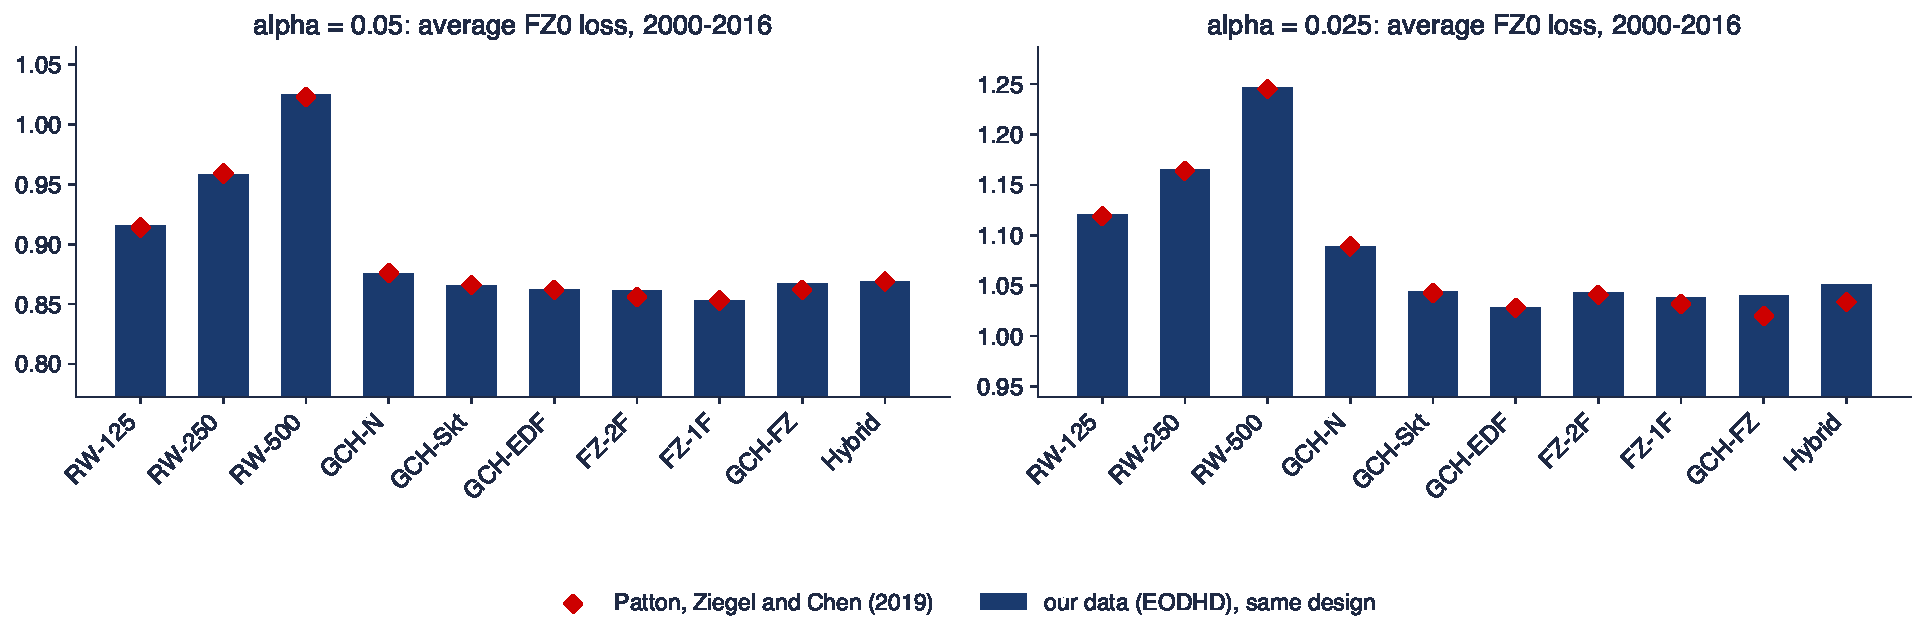
\includegraphics[width=0.97\textwidth,height=0.5\textheight,keepaspectratio]{ats_ch9_pzc_table.pdf}
\end{center}
\vspace{-0.25cm}
\begin{itemize}
    \item Average FZ0 loss of ten (VaR, ES) models, S\&P 500, 2000--2016, the design of \refPZC: our data (bars) against their Table 8 (diamonds)
\end{itemize}
\quantlet{ATS\_ch9\_pzc}{https://github.com/danpele/Advanced-Time-Series/tree/main/Quantlets/Ch_09/ATS_ch9_pzc}
\end{frame}

\begin{frame}{Interpreting the two kinds of outcome}
\itemsize{\small}
\begin{itemize}
    \item Average losses over 4\,000 days are robust to small data differences: GAS-1F 0.853 against 0.853
    \item Tests that rest on a few dozen tail days are not: goodness-of-fit $p$ = 0.001 against 0.242
    \item The same pattern in \atschlink{https://danpele.github.io/Advanced-Time-Series/EN/Courses/chapter2_structural_breaks_nonlinear_models.pdf}{Chapter 2} (\refTPS: $p$ = 0.165 against 0.002) and \atschlink{https://danpele.github.io/Advanced-Time-Series/EN/Courses/chapter14_causal_inference_time_series.pdf}{Chapter 14} (\refBMSS: $-$1.5\% against $-$2.4\%)
    \item Lesson: replicate the estimate and the inference separately; report which of the two survives
\end{itemize}
\end{frame}

\begin{frame}{Five sources of discrepancy}
\itemsize{\footnotesize}
\begin{itemize}
    \item \textbf{Data vintage}: revised GDP, rebased price indices, series that no longer exist
    \begin{itemize}
        \item Brexit gap (\atschlink{https://danpele.github.io/Advanced-Time-Series/EN/Courses/chapter14_causal_inference_time_series.pdf}{Chapter 14}), the UK CPI of TPS (\atschlink{https://danpele.github.io/Advanced-Time-Series/EN/Courses/chapter2_structural_breaks_nonlinear_models.pdf}{Chapter 2}), the decimals of MNZ (\atschlink{https://danpele.github.io/Advanced-Time-Series/EN/Courses/chapter6_state_space_models_bayesian_filtering.pdf}{Chapter 6})
    \end{itemize}
    \item \textbf{Sample}: the effect was a feature of its period
    \begin{itemize}
        \item the term spread (\atschlink{https://danpele.github.io/Advanced-Time-Series/EN/Courses/chapter0_refresher_inference.pdf}{Chapter 0}), diffusion indexes (\atschlink{https://danpele.github.io/Advanced-Time-Series/EN/Courses/chapter5_bvar_factor_models_nowcasting.pdf}{Chapter 5}), Hamilton's recessions (\atschlink{https://danpele.github.io/Advanced-Time-Series/EN/Courses/chapter7_regime_switching_models.pdf}{Chapter 7})
    \end{itemize}
    \item \textbf{Implementation}: optimiser, starting values, default options, the deterministic case
    \begin{itemize}
        \item EM maxima (\atschlink{https://danpele.github.io/Advanced-Time-Series/EN/Courses/chapter7_regime_switching_models.pdf}{Chapter 7}), the great ratios (\atschlink{https://danpele.github.io/Advanced-Time-Series/EN/Courses/chapter4_cointegration_vecm_ardl_panel.pdf}{Chapter 4}), diffuse initialisation (\atschlink{https://danpele.github.io/Advanced-Time-Series/EN/Courses/chapter6_state_space_models_bayesian_filtering.pdf}{Chapter 6})
    \end{itemize}
    \item \textbf{Inference}: the estimate survives, its standard error or critical value does not
    \begin{itemize}
        \item fixed-$b$ (\atschlink{https://danpele.github.io/Advanced-Time-Series/EN/Courses/chapter0_refresher_inference.pdf}{Chapter 0}), goodness-of-fit tests (\atschlink{https://danpele.github.io/Advanced-Time-Series/EN/Courses/chapter9_var_es_backtesting.pdf}{Chapter 9}), wild bootstrap (\atschlink{https://danpele.github.io/Advanced-Time-Series/EN/Courses/chapter16_explosive_roots_bubbles.pdf}{Chapter 16})
    \end{itemize}
    \item \textbf{Design}: the setting of the paper differs from yours
    \begin{itemize}
        \item dimension relative to sample for DCC-NL (\atschlink{https://danpele.github.io/Advanced-Time-Series/EN/Courses/chapter8_advanced_volatility.pdf}{Chapter 8}); the loss function for HARQ (\atschlink{https://danpele.github.io/Advanced-Time-Series/EN/Courses/chapter8_advanced_volatility.pdf}{Chapter 8})
    \end{itemize}
\end{itemize}
\end{frame}

\begin{frame}{How to replicate well}
\itemsize{\small}
\begin{itemize}
    \item Obtain the replication package; if none exists, write down every choice the paper leaves open
    \item Reproduce one number first (a coefficient, a test statistic), then the table, then the figure
    \item Keep the original sample as a separate run before extending it; change one thing at a time
    \item Use two implementations when possible (your code and a package), as for Hamilton's model in \atschlink{https://danpele.github.io/Advanced-Time-Series/EN/Courses/chapter7_regime_switching_models.pdf}{Chapter 7}
    \item Put published and replicated numbers side by side, with the absolute and relative differences
    \item A failed replication is a result: report the source of the difference, test the competing explanations, contact the authors politely if needed
\end{itemize}
\end{frame}


%=============================================================================
\section{The reproducibility checklist}
%=============================================================================

\begin{frame}{The repository}
\itemsize{\small}
\begin{center}
\scriptsize
\begin{tabular}{>{\raggedright\arraybackslash}p{5.4cm}>{\raggedright\arraybackslash}p{6.8cm}}
\toprule
\textbf{Path} & \textbf{Content} \\
\midrule
\texttt{README.md} & question, data statement, how to run, run time \\
\texttt{requirements.txt} & package versions \\
\texttt{data/raw/}, \texttt{data/processed/} & raw files never edited by hand \\
\texttt{code/01\_data.py}, \texttt{02\_replication.py}, \dots & numbered scripts, run in order \\
\texttt{notebooks/main.ipynb} & runs in Colab from start to end \\
\texttt{output/tables/}, \texttt{output/figures/} & generated by the code, never typed \\
\texttt{report/report.pdf} & the paper \\
\texttt{preregistration.md}, \texttt{AI\_USE.md}, \texttt{AI\_ERRORS.md} & the plan and the AI record \\
\bottomrule
\end{tabular}
\end{center}

\vspace{2mm}
\begin{itemize}
    \item The structure follows the data editors of economics journals \refVil; replication packages are now a condition of publication \refCM
    \item The preregistration.md file is committed before the first estimation commit: the history shows it
\end{itemize}
\end{frame}

\begin{frame}{Reproducibility checklist}
\itemsize{\small}
\begin{columns}[T]
\begin{column}{0.48\textwidth}
\begin{block}{Data and code}
\begin{itemize}
    \item every series: source, code, download date
    \item no manual step between raw data and results
    \item one command or one notebook runs everything
    \item random seeds fixed and reported; results stable across seeds
    \item functions tested on a case with a known answer (a simulated process, a published number)
\end{itemize}
\end{block}
\end{column}
\begin{column}{0.48\textwidth}
\begin{block}{Numbers and report}
\begin{itemize}
    \item every number in the report traceable to a file in output/
    \item package versions in requirements.txt
    \item the clean-machine test: a colleague clones and gets the same numbers \refPeng
    \item deviations from the pre-registration listed
    \item AI\_USE.md and AI\_ERRORS.md complete
\end{itemize}
\end{block}
\end{column}
\end{columns}
\end{frame}


%=============================================================================
\section{Failure modes}
%=============================================================================

\begin{frame}{Data snooping and p-hacking}
\itemsize{\small}
\begin{itemize}
    \item \textbf{Data snooping}: the same data are used to choose and to test a model; the reported $p$-value ignores the search \refWhite
    \begin{itemize}
        \item remedies: Reality Check, SPA \refHansen, StepM \refRW, MCS \refHLNa, a hold-out period never touched
    \end{itemize}
    \item \textbf{p-hacking}: undisclosed flexibility (samples, controls, transformations, outliers) until $p < 0.05$ \refSNS
    \begin{itemize}
        \item the ``garden of forking paths'': no conscious search is needed, data-dependent choices suffice \refGL
        \item published $z$-statistics bunch just above 1.96 \refBLSZ; in finance, a new factor needs $t > 3$ \refHLZ
    \end{itemize}
    \item Persistent predictors add a second problem: HAC tests over-reject, as in \atschlink{https://danpele.github.io/Advanced-Time-Series/EN/Courses/chapter0_refresher_inference.pdf}{Chapter 0} \refStam
\end{itemize}
\end{frame}

\begin{frame}{A specification search on a series with no predictability}
\itemsize{\footnotesize}
\begin{center}
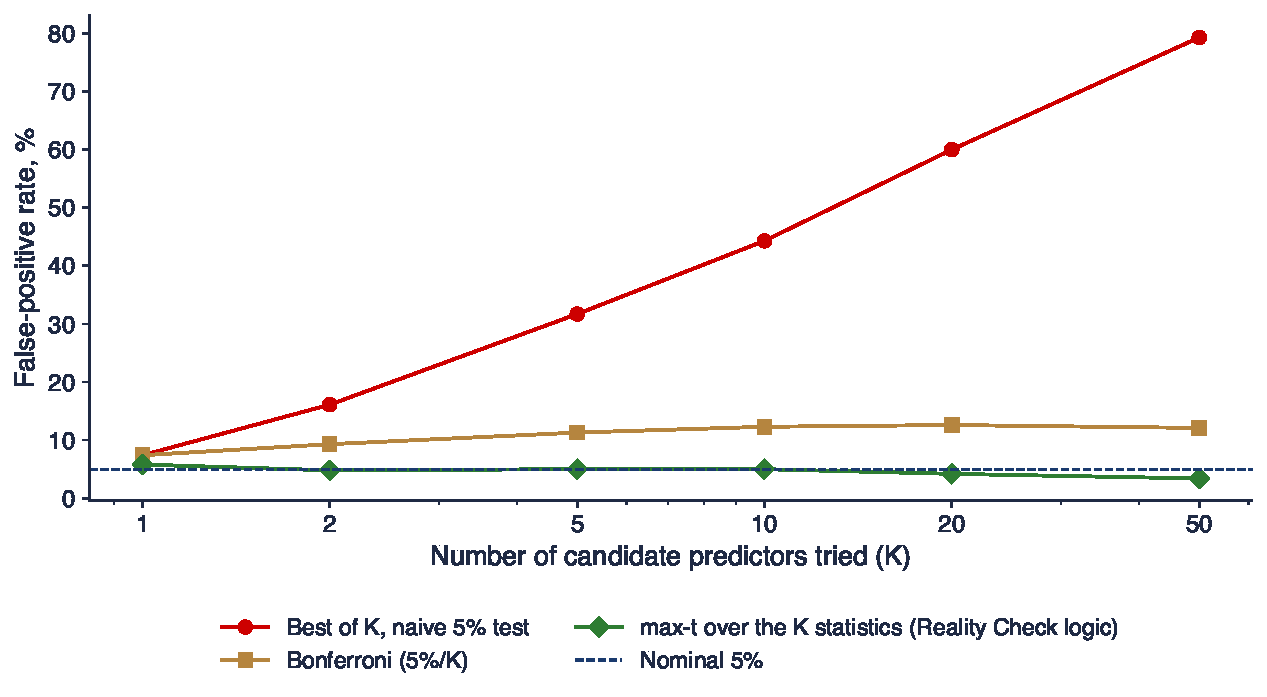
\includegraphics[width=0.97\textwidth,height=0.62\textheight,keepaspectratio]{ats_ch15_snooping.pdf}
\end{center}
\vspace{-0.25cm}
\begin{itemize}
    \item 1\,000 simulated data sets, $T$ = 250; $K$ persistent candidate predictors ($\rho = 0.9$, a common factor); HAC $t$-tests; the share of data sets with at least one ``discovery''
\end{itemize}
\quantlet{ATS\_ch15\_pitfalls}{https://github.com/danpele/Advanced-Time-Series/tree/main/Quantlets/Ch_15/ATS_ch15_pitfalls}
\end{frame}

\begin{frame}{Interpreting the specification search}
\itemsize{\small}
\begin{itemize}
    \item Reporting the best of $K$ as if it were the only one: 32\% false positives with 5 predictors, 60\% with 20, 79\% with 50
    \item Bonferroni does not fix it: 13\% at $K = 20$, because each HAC test is already oversized with persistent predictors (7\% at $K = 1$)
    \item The max-$t$ critical value simulated under the null with the same dependence keeps the rate near 5\%: 4\% at $K = 20$ (the logic of the Reality Check)
    \item The BET in \atschlink{https://danpele.github.io/Advanced-Time-Series/EN/Courses/chapter0_refresher_inference.pdf}{Chapter 0}: naive $p$ = 0.006, Reality Check $p$ = 0.06
    \item Pre-register $K$; report all $K$ results
\end{itemize}
\end{frame}

\begin{frame}{Leakage and look-ahead}
\itemsize{\small}
\begin{itemize}
    \item \textbf{Leakage}: information from the evaluation period enters the model \refKau
    \begin{itemize}
        \item selection of predictors, lags or hyperparameters on the whole sample
        \item scaling, detrending, filtering (HP, wavelets) or imputing with full-sample statistics
        \item random K-fold with dependent residuals or overlapping targets (\atschlink{https://danpele.github.io/Advanced-Time-Series/EN/Courses/chapter12_machine_learning_deep_learning.pdf}{Chapter 12})
    \end{itemize}
    \item \textbf{Look-ahead}: using data that were not available at the forecast date
    \begin{itemize}
        \item revised data instead of real-time vintages; publication lags ignored
        \item pretrained models whose training data cover the test period (\atschlink{https://danpele.github.io/Advanced-Time-Series/EN/Courses/chapter13_foundation_models_conformal.pdf}{Chapter 13})
    \end{itemize}
    \item Test: could I have computed this forecast on that date, with that information?
\end{itemize}
\end{frame}

\begin{frame}{Predictor selection with look-ahead}
\itemsize{\footnotesize}
\begin{center}
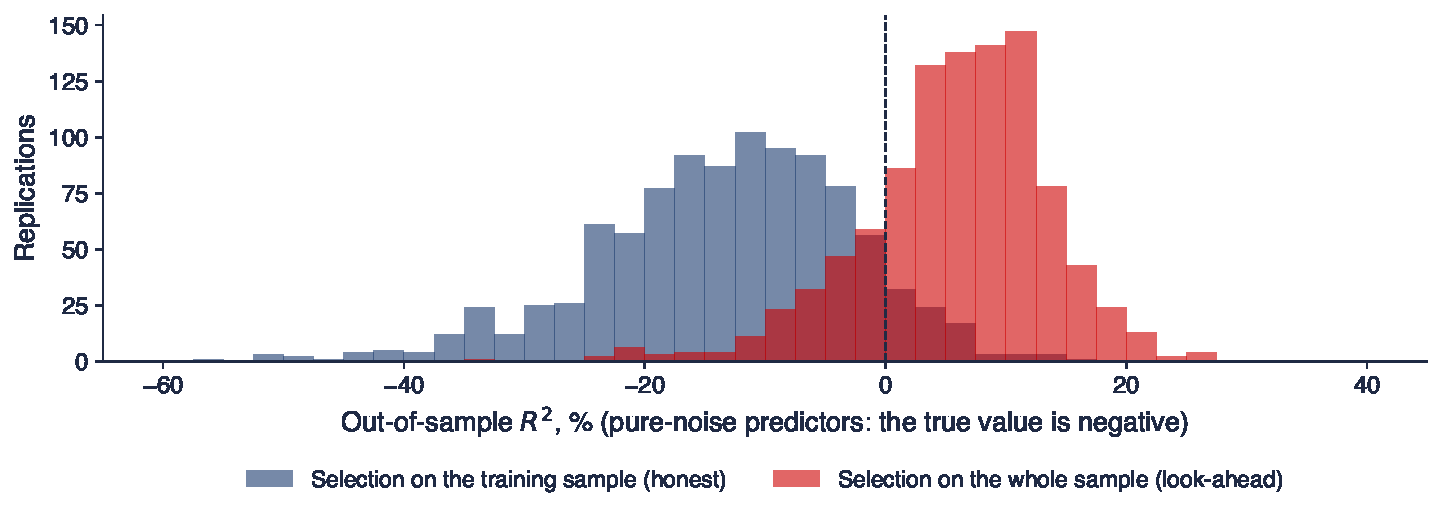
\includegraphics[width=0.97\textwidth,height=0.62\textheight,keepaspectratio]{ats_ch15_leakage.pdf}
\end{center}
\vspace{-0.25cm}
\begin{itemize}
    \item 1\,000 simulations: $T$ = 240, last 60 periods for testing, 100 pure-noise candidate predictors, the 5 most correlated kept, OLS on the training sample
\end{itemize}
\quantlet{ATS\_ch15\_pitfalls}{https://github.com/danpele/Advanced-Time-Series/tree/main/Quantlets/Ch_15/ATS_ch15_pitfalls}
\end{frame}

\begin{frame}{Interpreting the leakage experiment}
\itemsize{\small}
\begin{itemize}
    \item Honest selection: mean out-of-sample $R^2$ = \ensuremath{-}13.3\%, positive in 8\% of runs: noise does not forecast
    \item Selection on the whole sample: mean 5.9\%, positive in 81\% of runs: a ``forecasting gain'' created by the test period itself
    \item Out-of-sample evaluation protects you only if every choice is made inside the training window \refIK
    \item The same mechanism inflated the validation scores of \atschlink{https://danpele.github.io/Advanced-Time-Series/EN/Courses/chapter12_machine_learning_deep_learning.pdf}{Chapter 12} (ratio 0.34)
\end{itemize}
\end{frame}

\begin{frame}{Overclaiming}
\itemsize{\footnotesize}
\begin{columns}[T]
\begin{column}{0.58\textwidth}
\begin{itemize}
    \item \textbf{Causal language for predictive results}
    \begin{itemize}
        \item ``Granger-causes'' is not ``causes''; a common driver or timing produces it (\atschlink{https://danpele.github.io/Advanced-Time-Series/EN/Courses/chapter14_causal_inference_time_series.pdf}{Chapter 14})
    \end{itemize}
    \item \textbf{Significance for size}
    \begin{itemize}
        \item a significant DM test with a 0.3\% loss reduction is a small gain; report the effect and its interval
    \end{itemize}
    \item \textbf{Generality for one sample}
    \begin{itemize}
        \item one market, one period, one specification; say so in the title and the abstract
    \end{itemize}
    \item \textbf{Absence of evidence for evidence of absence}
    \begin{itemize}
        \item a non-rejection with low power says little: compute the power (Romanian nowcast, $p$ = 0.76)
    \end{itemize}
\end{itemize}
\end{column}
\begin{column}{0.38\textwidth}
\centering
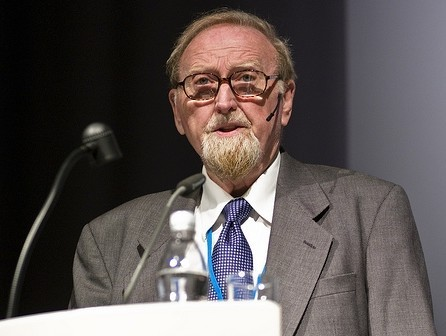
\includegraphics[height=0.40\textheight]{ch1_granger_2008.jpg}\\[1mm]
\imgcap{Clive Granger (2008)}
\imgcredit{https://commons.wikimedia.org/wiki/File:Clive_Granger_by_Olaf_Storbeck.jpg}{Photo: Olaf Storbeck (2008); CC BY-SA 2.0; Wikimedia Commons}
\end{column}
\end{columns}
\end{frame}

\begin{frame}{Recap: failure modes}
\itemsize{\small}
\begin{itemize}
    \item A search reported as a single test produces discoveries from noise; pre-register $K$ and correct for it
    \item Every choice inside the training window, every datum available at the forecast date
    \item Claims no stronger than the design: prediction is not causation, significance is not size
\end{itemize}
\end{frame}


%=============================================================================
\section{The oral defence}
%=============================================================================

\begin{frame}{Format of the defence}
\itemsize{\small}
\begin{columns}[T]
\begin{column}{0.6\textwidth}
\begin{itemize}
    \item Individual, about 15 minutes per student: each member is examined separately and receives a separate grade (50\% of the final grade)
    \item 5 minutes: presentation of one's own contribution, the part of the project the student led, on the report and the repository
    \item 10 minutes: questions on the code, the method and the results
    \begin{itemize}
        \item the code: open a file, explain a function, say what changes if a choice changes
        \item the method: the theory behind it, its assumptions and its alternatives
        \item the results: interpret a number, a test, a figure; defend the inference
    \end{itemize}
    \item Graded with the rubric on the next slide
    \item Every member must be able to answer questions on the whole project, not only on their part
    \item No AI tools during the defence; Romanian or English
\end{itemize}
\end{column}
\begin{column}{0.36\textwidth}
\centering
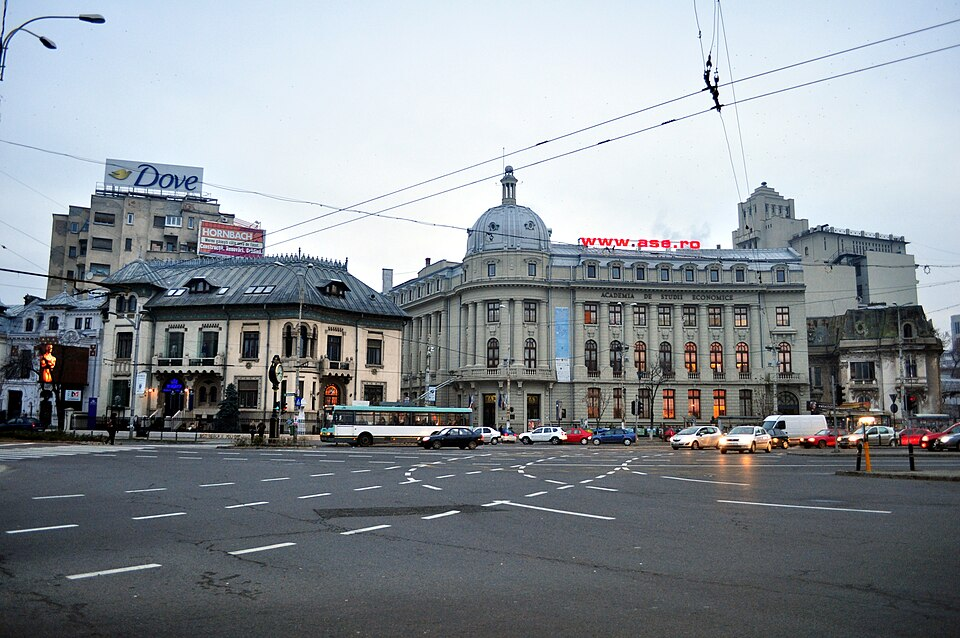
\includegraphics[height=0.36\textheight]{ch0_ase_2014.jpg}\\[1mm]
\imgcap{Bucharest University of Economic Studies}
\imgcredit{https://commons.wikimedia.org/wiki/File:Bucharest_-_Academie_de_Studii_Economice_01.jpg}{Photo: Joe Mabel (2014); CC BY 3.0; Wikimedia Commons}
\end{column}
\end{columns}
\end{frame}

\begin{frame}{Grading rubric of the individual defence}
\itemsize{\small}
\begin{center}
\scriptsize
\begin{tabular}{>{\raggedright\arraybackslash}p{3.4cm}>{\raggedright\arraybackslash}p{1.1cm}>{\raggedright\arraybackslash}p{8.2cm}}
\toprule
\textbf{Criterion} & \textbf{Points} & \textbf{What earns the points} \\
\midrule
Mastery of the method & 25 & states the model and its assumptions, derives the key result, knows when the method fails \\
Ownership of the code and data & 20 & explains any function of the repository, the data source and vintage, the effect of changing a setting \\
Inference and interpretation & 25 & valid standard errors for dependent data, effect sizes with intervals, correct reading of tests and of non-rejections \\
Replication and robustness & 20 & explains differences from the paper, the robustness design and the limits of the conclusion \\
Research integrity and AI use & 10 & describes what AI did, which errors were caught and how; deviations from the pre-registration \\
\bottomrule
\end{tabular}
\end{center}
\begin{itemize}
    \item The defence grade is the score out of 100 divided by 10; a member who cannot explain the code they submitted cannot pass
\end{itemize}
\end{frame}

\begin{frame}{What distinguishes the grades}
\itemsize{\small}
\begin{itemize}
    \item \textbf{9--10}
    \begin{itemize}
        \item answers ``why'' and ``what if'', not only ``what''; anticipates the weak points and has tested them
    \end{itemize}
    \item \textbf{7--8}
    \begin{itemize}
        \item correct methods and interpretation; hesitates on alternatives or on the asymptotics
    \end{itemize}
    \item \textbf{5--6}
    \begin{itemize}
        \item can run and describe the code; reads $p$-values mechanically; limited link to the theory
    \end{itemize}
    \item \textbf{below 5}
    \begin{itemize}
        \item cannot explain own code or numbers; claims not supported by the results; undeclared AI use
    \end{itemize}
\end{itemize}
\end{frame}

\begin{frame}{Typical questions with model answers (1/3): the code}
\itemsize{\footnotesize}
\begin{itemize}
    \item \textbf{Q}: Where in your code is the information set of the forecast for date $t$ fixed?
    \begin{itemize}
        \item \textbf{Model answer}: In the walk-forward loop: the estimation window ends at $t - h$, and scaling, selection and tuning are recomputed inside the loop (shows the lines)
    \end{itemize}
    \item \textbf{Q}: How many HAC lags do you use, and why?
    \begin{itemize}
        \item \textbf{Model answer}: The Newey--West rule $\lfloor 4(T/100)^{2/9}\rfloor$, at least $h - 1$ for overlapping $h$-step errors; the result is checked with fixed-$b$ critical values (\atschlink{https://danpele.github.io/Advanced-Time-Series/EN/Courses/chapter0_refresher_inference.pdf}{Chapter 0})
    \end{itemize}
    \item \textbf{Q}: What happens if you change the seed?
    \begin{itemize}
        \item \textbf{Model answer}: We reran with ten seeds: the ranking is unchanged, the loss changes by less than its standard error (a table in the report)
    \end{itemize}
\end{itemize}
\end{frame}

\begin{frame}{Typical questions with model answers (2/3): the results}
\itemsize{\footnotesize}
\begin{itemize}
    \item \textbf{Q}: Your DM test gives $p = 0.03$: is your model better?
    \begin{itemize}
        \item \textbf{Model answer}: Better in the pre-registered loss over this sample: the mean loss differential is X with a HAC interval; the models are not nested, so DM is valid; with several models we report the MCS
    \end{itemize}
    \item \textbf{Q}: Your replication differs from Table 2 of the paper. Why?
    \begin{itemize}
        \item \textbf{Model answer}: On the original sample we match to two decimals; the difference appears with the current data vintage, so it is revision, not code (shows the two runs)
    \end{itemize}
    \item \textbf{Q}: What result would have made you reject your hypothesis?
    \begin{itemize}
        \item \textbf{Model answer}: The pre-registration states it: a placebo date with a similar effect, or an effect that changes sign across the donor pools
    \end{itemize}
\end{itemize}
\end{frame}

\begin{frame}{Typical questions with model answers (3/3): the chapters}
\itemsize{\footnotesize}
\begin{itemize}
    \item \textbf{Q}: Why can you not use $\chi^2$ critical values to test two regimes against one?
    \begin{itemize}
        \item \textbf{Model answer}: Under the null the transition probabilities are not identified, a parameter is on the boundary and the score is zero: the bootstrap or Hansen's and Garcia's methods are needed (\atschlink{https://danpele.github.io/Advanced-Time-Series/EN/Courses/chapter7_regime_switching_models.pdf}{Chapter 7})
    \end{itemize}
    \item \textbf{Q}: Why is K-fold cross-validation acceptable for your AR model but not for your random forest?
    \begin{itemize}
        \item \textbf{Model answer}: For a well-specified autoregression the residuals are uncorrelated, so the folds are valid \refBHK; the forest's residuals are autocorrelated, so we block and purge (\atschlink{https://danpele.github.io/Advanced-Time-Series/EN/Courses/chapter12_machine_learning_deep_learning.pdf}{Chapter 12})
    \end{itemize}
    \item \textbf{Q}: Is a significant Granger test a causal effect?
    \begin{itemize}
        \item \textbf{Model answer}: No: it is predictive relative to an information set; a causal claim needs an identifying assumption about the assignment, such as an instrument or a synthetic control with placebos (\atschlink{https://danpele.github.io/Advanced-Time-Series/EN/Courses/chapter14_causal_inference_time_series.pdf}{Chapter 14})
    \end{itemize}
\end{itemize}
\end{frame}

\begin{frame}{Where defences go wrong}
\itemsize{\small}
\begin{itemize}
    \item Code written by someone else (a colleague or an AI assistant) that the presenter cannot explain
    \item A $p$-value read as the probability that the hypothesis is true
    \item A forecasting gain without a test, or a test without the size of the gain
    \item Not knowing the data: source, frequency, vintage, transformations, sample dates
    \item Numbers in the report that the repository does not reproduce
    \item Defending every result instead of explaining its limits
\end{itemize}
\end{frame}


%=============================================================================
\section{AI in research}
%=============================================================================

\begin{frame}{AI\_USE.md: what was asked and what was kept}
\itemsize{\small}
\begin{itemize}
    \item AI tools are allowed and declared; undeclared use counts as plagiarism
    \item For each use, one entry
    \begin{itemize}
        \item the tool and version, the date, the step of the workflow
        \item the prompt (or a faithful summary of it)
        \item what was kept, changed or rejected, and how it was checked
    \end{itemize}
    \item Useful uses
    \begin{itemize}
        \item literature search with verified DOIs; first drafts of code with tests; a hostile-referee critique of the design \refKor
    \end{itemize}
    \item Risky uses
    \begin{itemize}
        \item references, numbers and dates taken without checking \refWW; text that claims more than the results
        \item the illusion of understanding: fluent output mistaken for knowledge \refMC
    \end{itemize}
\end{itemize}
\end{frame}

\begin{frame}{AI\_ERRORS.md: at least three errors caught}
\itemsize{\small}
\begin{center}
\scriptsize
\begin{tabular}{>{\raggedright\arraybackslash}p{2.6cm}>{\raggedright\arraybackslash}p{5.0cm}>{\raggedright\arraybackslash}p{4.8cm}}
\toprule
\textbf{Type} & \textbf{Example from the course} & \textbf{How it is caught} \\
\midrule
invented reference & a plausible title with a DOI that resolves to another paper & Crossref lookup: title and authors must match \\
wrong formula & ES scored alone with a quantile loss (\atschlink{https://danpele.github.io/Advanced-Time-Series/EN/Courses/chapter9_var_es_backtesting.pdf}{Chapter 9}) & derivation on paper; a simulation with known answer \\
leakage in code & a scaler fitted on the whole sample before the split & the date test: recompute a forecast with data up to its date only \\
wrong default & a $\chi^2$ critical value for a sup-test (\atschlink{https://danpele.github.io/Advanced-Time-Series/EN/Courses/chapter2_structural_breaks_nonlinear_models.pdf}{Chapter 2}) & read the documentation and the paper; reproduce a published value \\
overclaiming & ``Granger causality proves that ...'' (\atschlink{https://danpele.github.io/Advanced-Time-Series/EN/Courses/chapter14_causal_inference_time_series.pdf}{Chapter 14}) & compare each sentence with the design \\
\bottomrule
\end{tabular}
\end{center}
\begin{itemize}
    \item Each entry: what the tool produced, why it was wrong, how it was detected, what replaced it
\end{itemize}
\end{frame}

\begin{frame}{A verification protocol}
\itemsize{\small}
\begin{itemize}
    \item References: every DOI resolved and the title matched; the claimed result found in the paper
    \item Code: run on a simulated process with known parameters before the real data; compare with a second implementation
    \item Numbers: every number in the report regenerated by the repository; none copied from a chat
    \item Dates and facts: from official sources (Eurostat, BNR, Monitorul Oficial), not from the model's memory
    \item Text: each claim checked against the design (prediction, association or causation)
    \item At the defence you explain everything yourself: what you cannot explain should not be in the project
\end{itemize}
\end{frame}


%=============================================================================
\section{AI for scientific discovery: choosing a project}
%=============================================================================

\begin{frame}{The open question}
\itemsize{\small}
\begin{itemize}
    \item \textbf{Which landmark results in time series econometrics survive on new data, and why do some not?}
    \begin{itemize}
        \item the course replications point to vintages, samples and inference; a systematic answer across papers does not exist
    \end{itemize}
    \item AI tools change the cost of each step
    \begin{itemize}
        \item literature maps and code drafts in hours \refWang; fully automated pipelines have been proposed \refLu
        \item the scarce resource becomes judgement: the design, the checks, the interpretation
    \end{itemize}
    \item Your project is one data point in this question: a replication with a clear verdict and a documented reason
\end{itemize}
\end{frame}

\begin{frame}{The discovery loop with an AI assistant}
\itemsize{\footnotesize}
\begin{itemize}
    \item An AI assistant (an LLM such as Claude, ChatGPT, Gemini or Copilot) speeds up each step; Semantic Scholar and Elicit help with the literature
    \begin{itemize}
        \item \textbf{literature}: \aiprompt{List replications of Meese and Rogoff (1983) for Central and Eastern European currencies since 2010, with DOIs, horizons and verdicts.} Then check every DOI
        \item \textbf{design}: \aiprompt{Given a loss differential with autocorrelation 0.3, how many out-of-sample months are needed for 80\% power to detect a mean gain of 0.2 standard deviations?}
        \item \textbf{code and replication}: ask for a DM--HLN function, then test it on simulated data with a known answer
        \item \textbf{critique}: \aiprompt{Act as a hostile referee of this pre-registration: where can the results leak into the design?}
    \end{itemize}
    \item Report: what was asked, what was kept, what was rejected (AI\_USE.md, AI\_ERRORS.md)
\end{itemize}
\end{frame}

\begin{frame}{What the human checks}
\itemsize{\small}
\begin{itemize}
    \item The paper exists, says what is claimed, and its data are available today
    \item The power calculation uses the dependence of your own loss differential, estimated on the training period
    \item The formula behind an AI answer: a power claim without the long-run variance is wrong for dependent data
    \item The extension is feasible in one semester with the course tools
    \item The verdict criteria (replicated, partly, not) are written before the replication is run
\end{itemize}
\end{frame}

\begin{frame}{Mini-case: is the evaluation sample long enough?}
\itemsize{\footnotesize}
\begin{center}
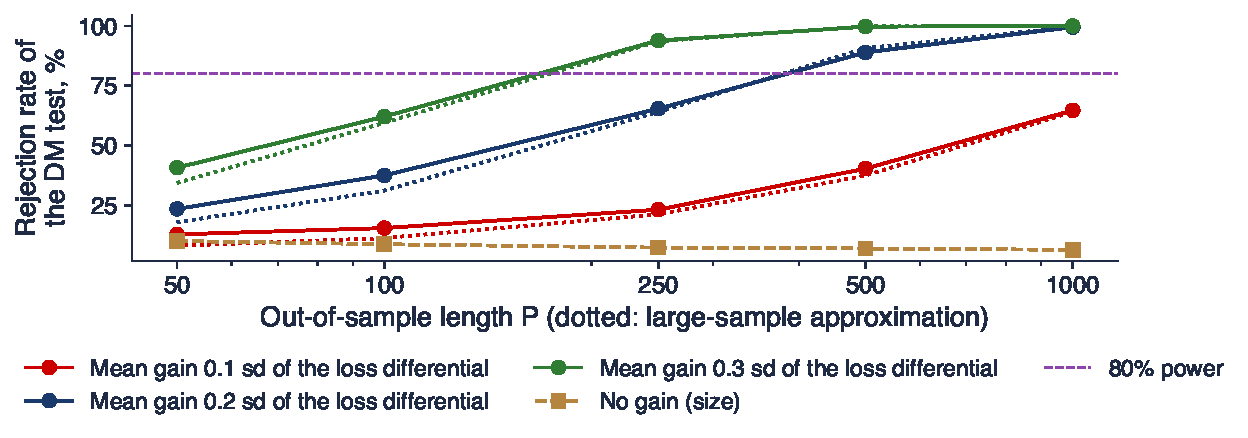
\includegraphics[width=0.97\textwidth,height=0.62\textheight,keepaspectratio]{ats_ch15_power.pdf}
\end{center}
\vspace{-0.25cm}
\begin{itemize}
    \item Rejection rate of the DM--HLN test (5\%, two-sided, 2\,000 simulations) when the loss differential is a mean gain plus an AR(1) with coefficient 0.3; dotted: $\Phi\big(\delta\sqrt{P/\Omega} - 1.96\big)$
\end{itemize}
\quantlet{ATS\_ch15\_power}{https://github.com/danpele/Advanced-Time-Series/tree/main/Quantlets/Ch_15/ATS_ch15_power}
\end{frame}

\begin{frame}{Interpreting the mini-case}
\itemsize{\small}
\begin{itemize}
    \item A gain of 0.2 standard deviations is detected with probability 38\% at $P = 100$ and 89\% at $P = 500$; 80\% power needs about 364 observations
    \item A gain of 0.1 needs about 1458: more than 120 years of monthly data; a gain of 0.3 about 162
    \item The rule $P \approx \Omega\,(z_{0.975} + z_{0.8})^2/\delta^2$ with $\Omega = (1 + \rho)/(1 - \rho)$ = 1.86: dependence multiplies the sample you need
    \item With few observations the test is also oversized: 10.1\% at $P = 50$
    \item Choose a question your data can answer: monthly macro data rarely detect small gains, daily or intraday data can
\end{itemize}
\end{frame}

\begin{frame}{Project idea}
\itemsize{\small}
\begin{itemize}
    \item \textbf{Choosing the project: four criteria}
    \begin{itemize}
        \item a landmark paper with public data or a precise data description, and a number to match
        \item an extension that answers one new question, preferably on Romanian or EU data
        \item enough power for the evaluation you plan (the mini-case)
        \item a verdict rule written before the first estimate
    \end{itemize}
    \item \textbf{Example}: why do some replications fail? A replication audit of three course papers
    \begin{itemize}
        \item replicate \refTPS, \refPZC{} and \refBMSS{} on the original and on today's data; attribute each difference to vintage, sample, implementation or inference
        \item extend: archived vintages (ALFRED, OECD Economic Outlook), a specification curve, a power analysis of each original test
    \end{itemize}
    \item Deliverables follow the course rules: repository, report, AI\_USE.md, AI\_ERRORS.md, oral defence
\end{itemize}
\end{frame}


%=============================================================================
\section{Wrap-up}
%=============================================================================

\begin{frame}{Key takeaways}
\itemsize{\small}
\begin{itemize}
    \item Five questions for every analysis: target, dependence, identification, evaluation, robustness
    \item Most landmark results replicate in direction; their strength and their tests depend on vintage, sample and inference
    \item Pre-register the design, compute the power, and make every number reproducible from one command
    \item Searches, leakage and look-ahead create discoveries from noise; causal words need causal designs
    \item The defence is individual: explain the method, the code, the inference and the limits yourself
\end{itemize}
\end{frame}

\begin{frame}{Self-assessment}
\itemsize{\small}
\begin{columns}[T]
\begin{column}{0.58\textwidth}
\begin{block}{Questions}
\begin{itemize}
    \item Which assumption identifies the main result of your project?
    \item How many specifications did you try, and how does your inference account for them?
    \item Could each forecast have been computed on its date?
    \item What is the power of your main test?
    \item Which of your numbers would change with a new data vintage?
\end{itemize}
\end{block}
\end{column}
\begin{column}{0.38\textwidth}
\begin{block}{Further study}
\begin{itemize}
    \item \refCM; \refCle; \refMen
    \item \refDiebold; \refLLSW
    \item Self-study \atschlink{https://danpele.github.io/Advanced-Time-Series/EN/Courses/chapter16_explosive_roots_bubbles.pdf}{Chapter 16} and its quiz
\end{itemize}
\end{block}
\end{column}
\end{columns}
\end{frame}


%=============================================================================
\section{Appendix}
%=============================================================================

\begin{frame}{Appendix: project seeds by chapter (1/2)}
\hypertarget{atsapp1}{}\atsappback{atssrc1}{Back}
\itemsize{\small}
\begin{center}
\scriptsize
\begin{tabular}{l>{\raggedright\arraybackslash}p{5.0cm}>{\raggedright\arraybackslash}p{6.6cm}}
\toprule
\textbf{Ch.} & \textbf{Replicate} & \textbf{Extend} \\
\midrule
0 & \refEH{} & the euro area and Romania; fixed-$b$ inference; stability across decades \\
1 & \refMR{} & CEE currencies, density forecasts, real-time macro fundamentals \\
2 & \refBP{} & breaks in Romanian inflation and the policy rate; real-time monitoring \\
3 & \refGK{} & ECB surprises and Romanian financial conditions with LP-IV \\
4 & \refPSS{} & interest-rate pass-through in the EU with CCE \\
5 & \refBGR{} & a large BVAR with stochastic volatility for Romania, nowcasting with news \\
6 & \refMNZ{} & the Romanian output gap and its real-time revisions \\
7 & \refHam{} & real-time recession probabilities for the euro area \\
8 & \refBPQ{} & HARQ for the BET and EUR/RON with realised measures \\
\bottomrule
\end{tabular}
\end{center}
\end{frame}

\begin{frame}{Appendix: project seeds by chapter (2/2)}
\hypertarget{atsapp2}{}\atsappback{atssrc1}{Back}
\itemsize{\small}
\begin{center}
\scriptsize
\begin{tabular}{l>{\raggedright\arraybackslash}p{5.0cm}>{\raggedright\arraybackslash}p{6.6cm}}
\toprule
\textbf{Ch.} & \textbf{Replicate} & \textbf{Extend} \\
\midrule
9 & \refPZC{} & CEE indices; the power of the backtests \\
10 & \refGJR{} & roughness of CEE and crypto volatility; robustness to noise \\
11 & \refCN, \refHamB{} & real-time output gaps of the EU members \\
12 & \refZeng{} & EU electricity load; global models; honest benchmarks \\
13 & \refGC{} & conformal VaR for the BET; coverage by regime \\
14 & \refADH, \refBMSS{} & tax and energy measures in CEE with synthetic controls \\
16 & \refPY{} & house prices and rents in EU capitals \\
15 & \refTPS, \refPZC, \refBMSS{} & a replication audit (the project idea of this chapter) \\
\bottomrule
\end{tabular}
\end{center}
\begin{itemize}
    \item Part C of every seminar contains a further project seed with its data
\end{itemize}
\end{frame}

\begin{frame}{Appendix: a pre-registration template}
\hypertarget{atsapp3}{}\atsappback{atssrc1}{Back}
\itemsize{\small}
\begin{itemize}
    \item \textbf{1. Question and hypotheses}: the primary hypothesis, in one sentence; secondary hypotheses
    \item \textbf{2. Paper to replicate}: the table or figure, the sample, what counts as ``replicated'', ``partly'', ``not replicated''
    \item \textbf{3. Data}: series, sources, vintage date, frequency, transformations, exclusions
    \item \textbf{4. Models}: benchmark and competitors, estimation method, how hyperparameters are chosen (inside the training window)
    \item \textbf{5. Evaluation}: windows (rolling or expanding), horizons, losses, tests, multiplicity correction, power calculation
    \item \textbf{6. Robustness}: the list of variations and the rule for a robust result
    \item \textbf{7. Team}: who leads which part (the basis of the individual defence)
\end{itemize}
\end{frame}


%=============================================================================
\section{References}
%=============================================================================

\begin{frame}{References (1/6)}
\itemsize{\tiny}
\begin{itemize}
    \item Abadie, A., Diamond, A., \& Hainmueller, J. (2015). Comparative politics and the synthetic control method. \textit{American Journal of Political Science}, 59(2), 495--510. \href{https://doi.org/10.1111/ajps.12116}{doi:10.1111/ajps.12116}
    \item Atkeson, A., \& Ohanian, L. E. (2001). Are Phillips curves useful for forecasting inflation? \textit{Federal Reserve Bank of Minneapolis Quarterly Review}, 25(1), 2--11. \href{https://doi.org/10.21034/qr.2511}{doi:10.21034/qr.2511}
    \item Bańbura, M., Giannone, D., \& Reichlin, L. (2010). Large Bayesian vector auto regressions. \textit{Journal of Applied Econometrics}, 25(1), 71--92. \href{https://doi.org/10.1002/jae.1137}{doi:10.1002/jae.1137}
    \item Bai, J., \& Perron, P. (2003). Computation and analysis of multiple structural change models. \textit{Journal of Applied Econometrics}, 18(1), 1--22. \href{https://doi.org/10.1002/jae.659}{doi:10.1002/jae.659}
    \item Bergmeir, C., Hyndman, R. J., \& Koo, B. (2018). A note on the validity of cross-validation for evaluating autoregressive time series prediction. \textit{Computational Statistics \& Data Analysis}, 120, 70--83. \href{https://doi.org/10.1016/j.csda.2017.11.003}{doi:10.1016/j.csda.2017.11.003}
    \item Bollerslev, T., Patton, A. J., \& Quaedvlieg, R. (2016). Exploiting the errors: A simple approach for improved volatility forecasting. \textit{Journal of Econometrics}, 192(1), 1--18. \href{https://doi.org/10.1016/j.jeconom.2015.10.007}{doi:10.1016/j.jeconom.2015.10.007}
    \item Born, B., Müller, G. J., Schularick, M., \& Sedláček, P. (2019). The costs of economic nationalism: Evidence from the Brexit experiment. \textit{The Economic Journal}, 129(623), 2722--2744. \href{https://doi.org/10.1093/ej/uez020}{doi:10.1093/ej/uez020}
    \item Brodeur, A., Lé, M., Sangnier, M., \& Zylberberg, Y. (2016). Star wars: The empirics strike back. \textit{American Economic Journal: Applied Economics}, 8(1), 1--32. \href{https://doi.org/10.1257/app.20150044}{doi:10.1257/app.20150044}
    \item Chang, A. C., \& Li, P. (2022). Is economics research replicable? Sixty published papers from thirteen journals say ``often not''. \textit{Critical Finance Review}, 11(1), 185--206. \href{https://doi.org/10.1561/104.00000053}{doi:10.1561/104.00000053}
    \item Christensen, G., \& Miguel, E. (2018). Transparency, reproducibility, and the credibility of economics research. \textit{Journal of Economic Literature}, 56(3), 920--980. \href{https://doi.org/10.1257/jel.20171350}{doi:10.1257/jel.20171350}
    \item Christiano, L. J., Eichenbaum, M., \& Evans, C. L. (1999). Monetary policy shocks: What have we learned and to what end? In J. B. Taylor \& M. Woodford (Eds.), \textit{Handbook of Macroeconomics}, Vol.\ 1A, 65--148. Elsevier. \href{https://doi.org/10.1016/S1574-0048(99)01005-8}{doi:10.1016/S1574-0048(99)01005-8}
    \item Clark, T. E., \& West, K. D. (2007). Approximately normal tests for equal predictive accuracy in nested models. \textit{Journal of Econometrics}, 138(1), 291--311. \href{https://doi.org/10.1016/j.jeconom.2006.05.023}{doi:10.1016/j.jeconom.2006.05.023}
    \item Clemens, M. A. (2017). The meaning of failed replications: A review and proposal. \textit{Journal of Economic Surveys}, 31(1), 326--342. \href{https://doi.org/10.1111/joes.12139}{doi:10.1111/joes.12139}
\end{itemize}
\end{frame}

\begin{frame}{References (2/6)}
\itemsize{\tiny}
\begin{itemize}
    \item Cogley, T., \& Nason, J. M. (1995). Effects of the Hodrick--Prescott filter on trend and difference stationary time series: Implications for business cycle research. \textit{Journal of Economic Dynamics and Control}, 19(1--2), 253--278. \href{https://doi.org/10.1016/0165-1889(93)00781-X}{doi:10.1016/0165-1889(93)00781-X}
    \item Diebold, F. X. (2015). Comparing predictive accuracy, twenty years later: A personal perspective on the use and abuse of Diebold--Mariano tests. \textit{Journal of Business \& Economic Statistics}, 33(1), 1--9. \href{https://doi.org/10.1080/07350015.2014.983236}{doi:10.1080/07350015.2014.983236}
    \item Diebold, F. X., \& Mariano, R. S. (1995). Comparing predictive accuracy. \textit{Journal of Business \& Economic Statistics}, 13(3), 253--263. \href{https://doi.org/10.1080/07350015.1995.10524599}{doi:10.1080/07350015.1995.10524599}
    \item Engle, R. F., Ghysels, E., \& Sohn, B. (2013). Stock market volatility and macroeconomic fundamentals. \textit{Review of Economics and Statistics}, 95(3), 776--797. \href{https://doi.org/10.1162/REST_a_00300}{doi:10.1162/REST\_a\_00300}
    \item Engle, R. F., Ledoit, O., \& Wolf, M. (2019). Large dynamic covariance matrices. \textit{Journal of Business \& Economic Statistics}, 37(2), 363--375. \href{https://doi.org/10.1080/07350015.2017.1345683}{doi:10.1080/07350015.2017.1345683}
    \item Engle, R. F., \& Manganelli, S. (2004). CAViaR: Conditional autoregressive value at risk by regression quantiles. \textit{Journal of Business \& Economic Statistics}, 22(4), 367--381. \href{https://doi.org/10.1198/073500104000000370}{doi:10.1198/073500104000000370}
    \item Estrella, A., \& Hardouvelis, G. A. (1991). The term structure as a predictor of real economic activity. \textit{The Journal of Finance}, 46(2), 555--576. \href{https://doi.org/10.1111/j.1540-6261.1991.tb02674.x}{doi:10.1111/j.1540-6261.1991.tb02674.x}
    \item Gatheral, J., Jaisson, T., \& Rosenbaum, M. (2018). Volatility is rough. \textit{Quantitative Finance}, 18(6), 933--949. \href{https://doi.org/10.1080/14697688.2017.1393551}{doi:10.1080/14697688.2017.1393551}
    \item Gelman, A., \& Loken, E. (2014). The statistical crisis in science. \textit{American Scientist}, 102(6), 460--465. \href{https://doi.org/10.1511/2014.111.460}{doi:10.1511/2014.111.460}
    \item Genre, V., Kenny, G., Meyler, A., \& Timmermann, A. (2013). Combining expert forecasts: Can anything beat the simple average? \textit{International Journal of Forecasting}, 29(1), 108--121. \href{https://doi.org/10.1016/j.ijforecast.2012.06.004}{doi:10.1016/j.ijforecast.2012.06.004}
    \item Gertler, M., \& Karadi, P. (2015). Monetary policy surprises, credit costs, and economic activity. \textit{American Economic Journal: Macroeconomics}, 7(1), 44--76. \href{https://doi.org/10.1257/mac.20130329}{doi:10.1257/mac.20130329}
    \item Gibbs, I., \& Candès, E. (2021). Adaptive conformal inference under distribution shift. \textit{Advances in Neural Information Processing Systems 34}; \textit{arXiv:2106.00170}. \href{https://arxiv.org/abs/2106.00170}{arxiv.org}
    \item Hamilton, J. D. (1989). A new approach to the economic analysis of nonstationary time series and the business cycle. \textit{Econometrica}, 57(2), 357--384. \href{https://doi.org/10.2307/1912559}{doi:10.2307/1912559}
\end{itemize}
\end{frame}

\begin{frame}{References (3/6)}
\itemsize{\tiny}
\begin{itemize}
    \item Hamilton, J. D. (2018). Why you should never use the Hodrick--Prescott filter. \textit{Review of Economics and Statistics}, 100(5), 831--843. \href{https://doi.org/10.1162/rest_a_00706}{doi:10.1162/rest\_a\_00706}
    \item Hansen, B. E. (1997). Inference in TAR models. \textit{Studies in Nonlinear Dynamics \& Econometrics}, 2(1), 1--14. \href{https://doi.org/10.2202/1558-3708.1024}{doi:10.2202/1558-3708.1024}
    \item Hansen, P. R. (2005). A test for superior predictive ability. \textit{Journal of Business \& Economic Statistics}, 23(4), 365--380. \href{https://doi.org/10.1198/073500105000000063}{doi:10.1198/073500105000000063}
    \item Hansen, P. R., Lunde, A., \& Nason, J. M. (2011). The model confidence set. \textit{Econometrica}, 79(2), 453--497. \href{https://doi.org/10.3982/ECTA5771}{doi:10.3982/ECTA5771}
    \item Harvey, C. R., Liu, Y., \& Zhu, H. (2016). \ldots\ and the cross-section of expected returns. \textit{Review of Financial Studies}, 29(1), 5--68. \href{https://doi.org/10.1093/rfs/hhv059}{doi:10.1093/rfs/hhv059}
    \item Harvey, D. I., Leybourne, S. J., Sollis, R., \& Taylor, A. M. R. (2016). Tests for explosive financial bubbles in the presence of non-stationary volatility. \textit{Journal of Empirical Finance}, 38, 548--574. \href{https://doi.org/10.1016/j.jempfin.2015.09.002}{doi:10.1016/j.jempfin.2015.09.002}
    \item Harvey, D., Leybourne, S., \& Newbold, P. (1997). Testing the equality of prediction mean squared errors. \textit{International Journal of Forecasting}, 13(2), 281--291. \href{https://doi.org/10.1016/S0169-2070(96)00719-4}{doi:10.1016/S0169-2070(96)00719-4}
    \item Herndon, T., Ash, M., \& Pollin, R. (2014). Does high public debt consistently stifle economic growth? A critique of Reinhart and Rogoff. \textit{Cambridge Journal of Economics}, 38(2), 257--279. \href{https://doi.org/10.1093/cje/bet075}{doi:10.1093/cje/bet075}
    \item Hou, K., Xue, C., \& Zhang, L. (2020). Replicating anomalies. \textit{Review of Financial Studies}, 33(5), 2019--2133. \href{https://doi.org/10.1093/rfs/hhy131}{doi:10.1093/rfs/hhy131}
    \item Inoue, A., \& Kilian, L. (2005). In-sample or out-of-sample tests of predictability: Which one should we use? \textit{Econometric Reviews}, 23(4), 371--402. \href{https://doi.org/10.1081/ETC-200040785}{doi:10.1081/ETC-200040785}
    \item Ioannidis, J. P. A. (2005). Why most published research findings are false. \textit{PLoS Medicine}, 2(8), e124. \href{https://doi.org/10.1371/journal.pmed.0020124}{doi:10.1371/journal.pmed.0020124}
    \item Kaufman, S., Rosset, S., Perlich, C., \& Stitelman, O. (2012). Leakage in data mining: Formulation, detection, and avoidance. \textit{ACM Transactions on Knowledge Discovery from Data}, 6(4), 15. \href{https://doi.org/10.1145/2382577.2382579}{doi:10.1145/2382577.2382579}
    \item Kiefer, N. M., \& Vogelsang, T. J. (2005). A new asymptotic theory for heteroskedasticity-autocorrelation robust tests. \textit{Econometric Theory}, 21(6), 1130--1164. \href{https://doi.org/10.1017/S0266466605050565}{doi:10.1017/S0266466605050565}
\end{itemize}
\end{frame}

\begin{frame}{References (4/6)}
\itemsize{\tiny}
\begin{itemize}
    \item Kilian, L. (2009). Not all oil price shocks are alike: Disentangling demand and supply shocks in the crude oil market. \textit{American Economic Review}, 99(3), 1053--1069. \href{https://doi.org/10.1257/aer.99.3.1053}{doi:10.1257/aer.99.3.1053}
    \item King, R. G., Plosser, C. I., Stock, J. H., \& Watson, M. W. (1991). Stochastic trends and economic fluctuations. \textit{American Economic Review}, 81(4), 819--840. \href{https://www.jstor.org/stable/2006644}{jstor.org}
    \item Korinek, A. (2023). Generative AI for economic research: Use cases and implications for economists. \textit{Journal of Economic Literature}, 61(4), 1281--1317. \href{https://doi.org/10.1257/jel.20231736}{doi:10.1257/jel.20231736}
    \item Lazarus, E., Lewis, D. J., Stock, J. H., \& Watson, M. W. (2018). HAR inference: Recommendations for practice. \textit{Journal of Business \& Economic Statistics}, 36(4), 541--559. \href{https://doi.org/10.1080/07350015.2018.1506926}{doi:10.1080/07350015.2018.1506926}
    \item Lu, C., Lu, C., Lange, R. T., Foerster, J., Clune, J., \& Ha, D. (2024). The AI Scientist: Towards fully automated open-ended scientific discovery. \textit{arXiv:2408.06292}. \href{https://arxiv.org/abs/2408.06292}{arxiv.org}
    \item McConnell, M. M., \& Perez-Quiros, G. (2000). Output fluctuations in the United States: What has changed since the early 1980's? \textit{American Economic Review}, 90(5), 1464--1476. \href{https://doi.org/10.1257/aer.90.5.1464}{doi:10.1257/aer.90.5.1464}
    \item Meese, R. A., \& Rogoff, K. (1983). Empirical exchange rate models of the seventies: Do they fit out of sample? \textit{Journal of International Economics}, 14(1--2), 3--24. \href{https://doi.org/10.1016/0022-1996(83)90017-X}{doi:10.1016/0022-1996(83)90017-X}
    \item Menkveld, A. J., Dreber, A., Holzmeister, F., Huber, J., Johannesson, M., Kirchler, M., et al.\ (2024). Nonstandard errors. \textit{The Journal of Finance}, 79(3), 2339--2390. \href{https://doi.org/10.1111/jofi.13337}{doi:10.1111/jofi.13337}
    \item Messeri, L., \& Crockett, M. J. (2024). Artificial intelligence and illusions of understanding in scientific research. \textit{Nature}, 627(8002), 49--58. \href{https://doi.org/10.1038/s41586-024-07146-0}{doi:10.1038/s41586-024-07146-0}
    \item Morley, J. C., Nelson, C. R., \& Zivot, E. (2003). Why are the Beveridge--Nelson and unobserved-components decompositions of GDP so different? \textit{Review of Economics and Statistics}, 85(2), 235--243. \href{https://doi.org/10.1162/003465303765299765}{doi:10.1162/003465303765299765}
    \item Newey, W. K., \& West, K. D. (1987). A simple, positive semi-definite, heteroskedasticity and autocorrelation consistent covariance matrix. \textit{Econometrica}, 55(3), 703--708. \href{https://doi.org/10.2307/1913610}{doi:10.2307/1913610}
    \item Nie, Y., Nguyen, N. H., Sinthong, P., \& Kalagnanam, J. (2023). A time series is worth 64 words: Long-term forecasting with Transformers. \textit{International Conference on Learning Representations}; \textit{arXiv:2211.14730}. \href{https://arxiv.org/abs/2211.14730}{arxiv.org}
    \item Nosek, B. A., Ebersole, C. R., DeHaven, A. C., \& Mellor, D. T. (2018). The preregistration revolution. \textit{Proceedings of the National Academy of Sciences}, 115(11), 2600--2606. \href{https://doi.org/10.1073/pnas.1708274114}{doi:10.1073/pnas.1708274114}
\end{itemize}
\end{frame}

\begin{frame}{References (5/6)}
\itemsize{\tiny}
\begin{itemize}
    \item Patton, A. J., Ziegel, J. F., \& Chen, R. (2019). Dynamic semiparametric models for expected shortfall (and Value-at-Risk). \textit{Journal of Econometrics}, 211(2), 388--413. \href{https://doi.org/10.1016/j.jeconom.2018.10.008}{doi:10.1016/j.jeconom.2018.10.008}
    \item Peng, R. D. (2011). Reproducible research in computational science. \textit{Science}, 334(6060), 1226--1227. \href{https://doi.org/10.1126/science.1213847}{doi:10.1126/science.1213847}
    \item Pesaran, M. H., Shin, Y., \& Smith, R. P. (1999). Pooled mean group estimation of dynamic heterogeneous panels. \textit{Journal of the American Statistical Association}, 94(446), 621--634. \href{https://doi.org/10.1080/01621459.1999.10474156}{doi:10.1080/01621459.1999.10474156}
    \item Petropoulos, F., Apiletti, D., Assimakopoulos, V., Babai, M. Z., Barrow, D. K., Ben Taieb, S., et al.\ (2022). Forecasting: theory and practice. \textit{International Journal of Forecasting}, 38(3), 705--871. \href{https://doi.org/10.1016/j.ijforecast.2021.11.001}{doi:10.1016/j.ijforecast.2021.11.001}
    \item Phillips, P. C. B., Shi, S., \& Yu, J. (2015). Testing for multiple bubbles: Historical episodes of exuberance and collapse in the S\&P 500. \textit{International Economic Review}, 56(4), 1043--1078. \href{https://doi.org/10.1111/iere.12132}{doi:10.1111/iere.12132}
    \item Phillips, P. C. B., Wu, Y., \& Yu, J. (2011). Explosive behavior in the 1990s Nasdaq: When did exuberance escalate asset values? \textit{International Economic Review}, 52(1), 201--226. \href{https://doi.org/10.1111/j.1468-2354.2010.00625.x}{doi:10.1111/j.1468-2354.2010.00625.x}
    \item Phillips, P. C. B., \& Yu, J. (2011). Dating the timeline of financial bubbles during the subprime crisis. \textit{Quantitative Economics}, 2(3), 455--491. \href{https://doi.org/10.3982/QE82}{doi:10.3982/QE82}
    \item Qu, Z. (2011). A test against spurious long memory. \textit{Journal of Business \& Economic Statistics}, 29(3), 423--438. \href{https://doi.org/10.1198/jbes.2010.09153}{doi:10.1198/jbes.2010.09153}
    \item Romano, J. P., \& Wolf, M. (2005). Stepwise multiple testing as formalized data snooping. \textit{Econometrica}, 73(4), 1237--1282. \href{https://doi.org/10.1111/j.1468-0262.2005.00615.x}{doi:10.1111/j.1468-0262.2005.00615.x}
    \item Romano, Y., Patterson, E., \& Candès, E. (2019). Conformalized quantile regression. \textit{Advances in Neural Information Processing Systems 32}; \textit{arXiv:1905.03222}. \href{https://arxiv.org/abs/1905.03222}{arxiv.org}
    \item Silberzahn, R., Uhlmann, E. L., Martin, D. P., Anselmi, P., Aust, F., Awtrey, E., et al.\ (2018). Many analysts, one data set: Making transparent how variations in analytic choices affect results. \textit{Advances in Methods and Practices in Psychological Science}, 1(3), 337--356. \href{https://doi.org/10.1177/2515245917747646}{doi:10.1177/2515245917747646}
    \item Simmons, J. P., Nelson, L. D., \& Simonsohn, U. (2011). False-positive psychology: Undisclosed flexibility in data collection and analysis allows presenting anything as significant. \textit{Psychological Science}, 22(11), 1359--1366. \href{https://doi.org/10.1177/0956797611417632}{doi:10.1177/0956797611417632}
    \item Simonsohn, U., Simmons, J. P., \& Nelson, L. D. (2020). Specification curve analysis. \textit{Nature Human Behaviour}, 4(11), 1208--1214. \href{https://doi.org/10.1038/s41562-020-0912-z}{doi:10.1038/s41562-020-0912-z}
\end{itemize}
\end{frame}

\begin{frame}{References (6/6)}
\itemsize{\tiny}
\begin{itemize}
    \item Stambaugh, R. F. (1999). Predictive regressions. \textit{Journal of Financial Economics}, 54(3), 375--421. \href{https://doi.org/10.1016/S0304-405X(99)00041-0}{doi:10.1016/S0304-405X(99)00041-0}
    \item Steegen, S., Tuerlinckx, F., Gelman, A., \& Vanpaemel, W. (2016). Increasing transparency through a multiverse analysis. \textit{Perspectives on Psychological Science}, 11(5), 702--712. \href{https://doi.org/10.1177/1745691616658637}{doi:10.1177/1745691616658637}
    \item Stock, J. H., \& Watson, M. W. (2002). Macroeconomic forecasting using diffusion indexes. \textit{Journal of Business \& Economic Statistics}, 20(2), 147--162. \href{https://doi.org/10.1198/073500102317351921}{doi:10.1198/073500102317351921}
    \item Taylor, M. P., Peel, D. A., \& Sarno, L. (2001). Nonlinear mean-reversion in real exchange rates: Toward a solution to the purchasing power parity puzzles. \textit{International Economic Review}, 42(4), 1015--1042. \href{https://doi.org/10.1111/1468-2354.00144}{doi:10.1111/1468-2354.00144}
    \item Vilhuber, L. (2020). Reproducibility and replicability in economics. \textit{Harvard Data Science Review}, 2(4). \href{https://doi.org/10.1162/99608f92.4f6b9e67}{doi:10.1162/99608f92.4f6b9e67}
    \item Walters, W. H., \& Wilder, E. I. (2023). Fabrication and errors in the bibliographic citations generated by ChatGPT. \textit{Scientific Reports}, 13, 14045. \href{https://doi.org/10.1038/s41598-023-41032-5}{doi:10.1038/s41598-023-41032-5}
    \item Wang, H., Fu, T., Du, Y., Gao, W., Huang, K., Liu, Z., et al.\ (2023). Scientific discovery in the age of artificial intelligence. \textit{Nature}, 620(7972), 47--60. \href{https://doi.org/10.1038/s41586-023-06221-2}{doi:10.1038/s41586-023-06221-2}
    \item Welch, I., \& Goyal, A. (2008). A comprehensive look at the empirical performance of equity premium prediction. \textit{Review of Financial Studies}, 21(4), 1455--1508. \href{https://doi.org/10.1093/rfs/hhm014}{doi:10.1093/rfs/hhm014}
    \item White, H. (2000). A reality check for data snooping. \textit{Econometrica}, 68(5), 1097--1126. \href{https://doi.org/10.1111/1468-0262.00152}{doi:10.1111/1468-0262.00152}
    \item Zeng, A., Chen, M., Zhang, L., \& Xu, Q. (2023). Are Transformers effective for time series forecasting? \textit{Proceedings of the AAAI Conference on Artificial Intelligence}, 37(9), 11121--11128. \href{https://doi.org/10.1609/aaai.v37i9.26317}{doi:10.1609/aaai.v37i9.26317}
\end{itemize}
\end{frame}

\end{document}
